% Options for packages loaded elsewhere
\PassOptionsToPackage{unicode}{hyperref}
\PassOptionsToPackage{hyphens}{url}
\PassOptionsToPackage{dvipsnames,svgnames,x11names}{xcolor}
%
\documentclass[
  letterpaper,
  DIV=11,
  numbers=noendperiod]{scrartcl}

\usepackage{amsmath,amssymb}
\usepackage{lmodern}
\usepackage{iftex}
\ifPDFTeX
  \usepackage[T1]{fontenc}
  \usepackage[utf8]{inputenc}
  \usepackage{textcomp} % provide euro and other symbols
\else % if luatex or xetex
  \usepackage{unicode-math}
  \defaultfontfeatures{Scale=MatchLowercase}
  \defaultfontfeatures[\rmfamily]{Ligatures=TeX,Scale=1}
\fi
% Use upquote if available, for straight quotes in verbatim environments
\IfFileExists{upquote.sty}{\usepackage{upquote}}{}
\IfFileExists{microtype.sty}{% use microtype if available
  \usepackage[]{microtype}
  \UseMicrotypeSet[protrusion]{basicmath} % disable protrusion for tt fonts
}{}
\makeatletter
\@ifundefined{KOMAClassName}{% if non-KOMA class
  \IfFileExists{parskip.sty}{%
    \usepackage{parskip}
  }{% else
    \setlength{\parindent}{0pt}
    \setlength{\parskip}{6pt plus 2pt minus 1pt}}
}{% if KOMA class
  \KOMAoptions{parskip=half}}
\makeatother
\usepackage{xcolor}
\setlength{\emergencystretch}{3em} % prevent overfull lines
\setcounter{secnumdepth}{-\maxdimen} % remove section numbering
% Make \paragraph and \subparagraph free-standing
\ifx\paragraph\undefined\else
  \let\oldparagraph\paragraph
  \renewcommand{\paragraph}[1]{\oldparagraph{#1}\mbox{}}
\fi
\ifx\subparagraph\undefined\else
  \let\oldsubparagraph\subparagraph
  \renewcommand{\subparagraph}[1]{\oldsubparagraph{#1}\mbox{}}
\fi

\usepackage{color}
\usepackage{fancyvrb}
\newcommand{\VerbBar}{|}
\newcommand{\VERB}{\Verb[commandchars=\\\{\}]}
\DefineVerbatimEnvironment{Highlighting}{Verbatim}{commandchars=\\\{\}}
% Add ',fontsize=\small' for more characters per line
\usepackage{framed}
\definecolor{shadecolor}{RGB}{241,243,245}
\newenvironment{Shaded}{\begin{snugshade}}{\end{snugshade}}
\newcommand{\AlertTok}[1]{\textcolor[rgb]{0.68,0.00,0.00}{#1}}
\newcommand{\AnnotationTok}[1]{\textcolor[rgb]{0.37,0.37,0.37}{#1}}
\newcommand{\AttributeTok}[1]{\textcolor[rgb]{0.40,0.45,0.13}{#1}}
\newcommand{\BaseNTok}[1]{\textcolor[rgb]{0.68,0.00,0.00}{#1}}
\newcommand{\BuiltInTok}[1]{\textcolor[rgb]{0.00,0.23,0.31}{#1}}
\newcommand{\CharTok}[1]{\textcolor[rgb]{0.13,0.47,0.30}{#1}}
\newcommand{\CommentTok}[1]{\textcolor[rgb]{0.37,0.37,0.37}{#1}}
\newcommand{\CommentVarTok}[1]{\textcolor[rgb]{0.37,0.37,0.37}{\textit{#1}}}
\newcommand{\ConstantTok}[1]{\textcolor[rgb]{0.56,0.35,0.01}{#1}}
\newcommand{\ControlFlowTok}[1]{\textcolor[rgb]{0.00,0.23,0.31}{#1}}
\newcommand{\DataTypeTok}[1]{\textcolor[rgb]{0.68,0.00,0.00}{#1}}
\newcommand{\DecValTok}[1]{\textcolor[rgb]{0.68,0.00,0.00}{#1}}
\newcommand{\DocumentationTok}[1]{\textcolor[rgb]{0.37,0.37,0.37}{\textit{#1}}}
\newcommand{\ErrorTok}[1]{\textcolor[rgb]{0.68,0.00,0.00}{#1}}
\newcommand{\ExtensionTok}[1]{\textcolor[rgb]{0.00,0.23,0.31}{#1}}
\newcommand{\FloatTok}[1]{\textcolor[rgb]{0.68,0.00,0.00}{#1}}
\newcommand{\FunctionTok}[1]{\textcolor[rgb]{0.28,0.35,0.67}{#1}}
\newcommand{\ImportTok}[1]{\textcolor[rgb]{0.00,0.46,0.62}{#1}}
\newcommand{\InformationTok}[1]{\textcolor[rgb]{0.37,0.37,0.37}{#1}}
\newcommand{\KeywordTok}[1]{\textcolor[rgb]{0.00,0.23,0.31}{#1}}
\newcommand{\NormalTok}[1]{\textcolor[rgb]{0.00,0.23,0.31}{#1}}
\newcommand{\OperatorTok}[1]{\textcolor[rgb]{0.37,0.37,0.37}{#1}}
\newcommand{\OtherTok}[1]{\textcolor[rgb]{0.00,0.23,0.31}{#1}}
\newcommand{\PreprocessorTok}[1]{\textcolor[rgb]{0.68,0.00,0.00}{#1}}
\newcommand{\RegionMarkerTok}[1]{\textcolor[rgb]{0.00,0.23,0.31}{#1}}
\newcommand{\SpecialCharTok}[1]{\textcolor[rgb]{0.37,0.37,0.37}{#1}}
\newcommand{\SpecialStringTok}[1]{\textcolor[rgb]{0.13,0.47,0.30}{#1}}
\newcommand{\StringTok}[1]{\textcolor[rgb]{0.13,0.47,0.30}{#1}}
\newcommand{\VariableTok}[1]{\textcolor[rgb]{0.07,0.07,0.07}{#1}}
\newcommand{\VerbatimStringTok}[1]{\textcolor[rgb]{0.13,0.47,0.30}{#1}}
\newcommand{\WarningTok}[1]{\textcolor[rgb]{0.37,0.37,0.37}{\textit{#1}}}

\providecommand{\tightlist}{%
  \setlength{\itemsep}{0pt}\setlength{\parskip}{0pt}}\usepackage{longtable,booktabs,array}
\usepackage{calc} % for calculating minipage widths
% Correct order of tables after \paragraph or \subparagraph
\usepackage{etoolbox}
\makeatletter
\patchcmd\longtable{\par}{\if@noskipsec\mbox{}\fi\par}{}{}
\makeatother
% Allow footnotes in longtable head/foot
\IfFileExists{footnotehyper.sty}{\usepackage{footnotehyper}}{\usepackage{footnote}}
\makesavenoteenv{longtable}
\usepackage{graphicx}
\makeatletter
\def\maxwidth{\ifdim\Gin@nat@width>\linewidth\linewidth\else\Gin@nat@width\fi}
\def\maxheight{\ifdim\Gin@nat@height>\textheight\textheight\else\Gin@nat@height\fi}
\makeatother
% Scale images if necessary, so that they will not overflow the page
% margins by default, and it is still possible to overwrite the defaults
% using explicit options in \includegraphics[width, height, ...]{}
\setkeys{Gin}{width=\maxwidth,height=\maxheight,keepaspectratio}
% Set default figure placement to htbp
\makeatletter
\def\fps@figure{htbp}
\makeatother

\KOMAoption{captions}{tableheading}
\makeatletter
\makeatother
\makeatletter
\makeatother
\makeatletter
\@ifpackageloaded{caption}{}{\usepackage{caption}}
\AtBeginDocument{%
\ifdefined\contentsname
  \renewcommand*\contentsname{Table of contents}
\else
  \newcommand\contentsname{Table of contents}
\fi
\ifdefined\listfigurename
  \renewcommand*\listfigurename{List of Figures}
\else
  \newcommand\listfigurename{List of Figures}
\fi
\ifdefined\listtablename
  \renewcommand*\listtablename{List of Tables}
\else
  \newcommand\listtablename{List of Tables}
\fi
\ifdefined\figurename
  \renewcommand*\figurename{Figure}
\else
  \newcommand\figurename{Figure}
\fi
\ifdefined\tablename
  \renewcommand*\tablename{Table}
\else
  \newcommand\tablename{Table}
\fi
}
\@ifpackageloaded{float}{}{\usepackage{float}}
\floatstyle{ruled}
\@ifundefined{c@chapter}{\newfloat{codelisting}{h}{lop}}{\newfloat{codelisting}{h}{lop}[chapter]}
\floatname{codelisting}{Listing}
\newcommand*\listoflistings{\listof{codelisting}{List of Listings}}
\makeatother
\makeatletter
\@ifpackageloaded{caption}{}{\usepackage{caption}}
\@ifpackageloaded{subcaption}{}{\usepackage{subcaption}}
\makeatother
\makeatletter
\@ifpackageloaded{tcolorbox}{}{\usepackage[many]{tcolorbox}}
\makeatother
\makeatletter
\@ifundefined{shadecolor}{\definecolor{shadecolor}{rgb}{.97, .97, .97}}
\makeatother
\makeatletter
\makeatother
\ifLuaTeX
  \usepackage{selnolig}  % disable illegal ligatures
\fi
\IfFileExists{bookmark.sty}{\usepackage{bookmark}}{\usepackage{hyperref}}
\IfFileExists{xurl.sty}{\usepackage{xurl}}{} % add URL line breaks if available
\urlstyle{same} % disable monospaced font for URLs
\hypersetup{
  pdftitle={possible-render-issue},
  colorlinks=true,
  linkcolor={blue},
  filecolor={Maroon},
  citecolor={Blue},
  urlcolor={Blue},
  pdfcreator={LaTeX via pandoc}}

\title{possible-render-issue}
\author{}
\date{}

\begin{document}
\maketitle
\ifdefined\Shaded\renewenvironment{Shaded}{\begin{tcolorbox}[boxrule=0pt, enhanced, borderline west={3pt}{0pt}{shadecolor}, breakable, interior hidden, sharp corners, frame hidden]}{\end{tcolorbox}}\fi

\begin{Shaded}
\begin{Highlighting}[]
\ImportTok{using} \BuiltInTok{Distributions}
\ImportTok{using} \BuiltInTok{Plots}
\ImportTok{using} \BuiltInTok{PlotThemes; }\FunctionTok{theme}\NormalTok{(}\OperatorTok{:}\NormalTok{dracula)}
\end{Highlighting}
\end{Shaded}

\begin{Shaded}
\begin{Highlighting}[]
\NormalTok{v }\OperatorTok{=} \FunctionTok{rand}\NormalTok{(}\FunctionTok{Normal}\NormalTok{(}\FloatTok{5}\NormalTok{, }\FloatTok{1.5}\NormalTok{), }\FloatTok{1000}\NormalTok{)}

\FunctionTok{histogram}\NormalTok{(v)}
\end{Highlighting}
\end{Shaded}

\begin{figure}[H]

{\centering 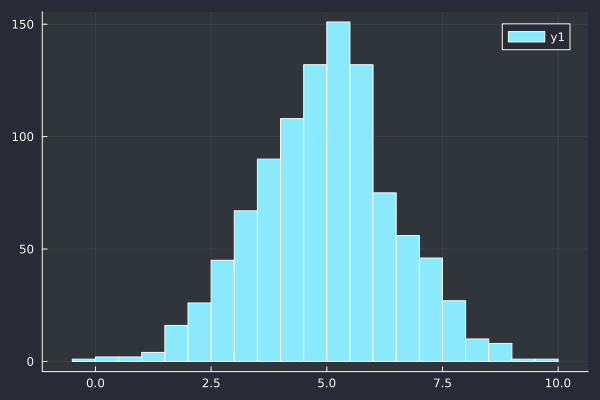
\includegraphics{Possible-render-issue_files/figure-pdf/cell-3-output-1.svg}

}

\end{figure}

If I uncomment the theme, I get:

\begin{Shaded}
\begin{Highlighting}[]
\NormalTok{\textasciitilde{}:) quarto render Possible{-}render{-}issue.qmd {-}{-}to pdf}

\NormalTok{Executing \textquotesingle{}Possible{-}render{-}issue.ipynb\textquotesingle{}}
\NormalTok{  Cell 1/2...Done}
\NormalTok{  Cell 2/2...Done}

\NormalTok{pandoc }
\NormalTok{  to: latex}
\NormalTok{  output{-}file: Possible{-}render{-}issue.tex}
\NormalTok{  standalone: true}
\NormalTok{  pdf{-}engine: xelatex}
\NormalTok{  variables:}
\NormalTok{    graphics: true}
\NormalTok{    tables: true}
\NormalTok{  default{-}image{-}extension: pdf}
  
\NormalTok{metadata}
\NormalTok{  documentclass: scrartcl}
\NormalTok{  classoption:}
\NormalTok{    {-} DIV=11}
\NormalTok{    {-} numbers=noendperiod}
\NormalTok{  papersize: letter}
\NormalTok{  header{-}includes:}
\NormalTok{    {-} \textquotesingle{}\textbackslash{}KOMAoption\{captions\}\{tableheading\}\textquotesingle{}}
\NormalTok{  block{-}headings: true}
\NormalTok{  title: Possible{-}render{-}issue}
  
\NormalTok{running xelatex {-} 1}
\NormalTok{  This is XeTeX, Version 3.141592653{-}2.6{-}0.999993 (TeX Live 2021) (preloaded format=xelatex)}
\NormalTok{   restricted \textbackslash{}write18 enabled.}
\NormalTok{  entering extended mode}
  
\NormalTok{updating tlmgr}

\NormalTok{updating existing packages}

\NormalTok{compilation failed{-} error}
\NormalTok{LaTeX Error: Cannot determine size of graphic in Possible{-}render{-}issue\_files/}
\NormalTok{figure{-}pdf/cell{-}3{-}output{-}1.svg (no BoundingBox).}

\NormalTok{See the LaTeX manual or LaTeX Companion for explanation.}
\NormalTok{Type  H \textless{}return\textgreater{}  for immediate help.}
\NormalTok{ ...                                              }
                                                  
\NormalTok{l.211 ...sue\_files/figure{-}pdf/cell{-}3{-}output{-}1.svg\}}
                                                   

\NormalTok{see /home/thadryan/Workspace/possible{-}render{-}issue/Possible{-}render{-}issue.log for more information}
\end{Highlighting}
\end{Shaded}

When I open that, I see:

\begin{Shaded}
\begin{Highlighting}[]
\NormalTok{This is XeTeX, Version 3.141592653{-}2.6{-}0.999993 (TeX Live 2021) (preloaded format=xelatex 2023.1.19)  30 JAN 2023 10:40}
\NormalTok{entering extended mode}
\NormalTok{ restricted \textbackslash{}write18 enabled.}
\NormalTok{ \%\&{-}line parsing enabled.}
\NormalTok{**Possible{-}render{-}issue.tex}
\NormalTok{(./Possible{-}render{-}issue.tex}
\NormalTok{LaTeX2e \textless{}2020{-}10{-}01\textgreater{} patch level 4}
\NormalTok{L3 programming layer \textless{}2021{-}05{-}07\textgreater{} (/usr/share/texlive/texmf{-}dist/tex/latex/koma}
\NormalTok{{-}script/scrartcl.cls}
\NormalTok{Document Class: scrartcl 2021/03/17 v3.33 KOMA{-}Script document class (article)}
\NormalTok{(/usr/share/texlive/texmf{-}dist/tex/latex/koma{-}script/scrkbase.sty}
\NormalTok{Package: scrkbase 2021/03/17 v3.33 KOMA{-}Script package (KOMA{-}Script{-}dependent b}
\NormalTok{asics and keyval usage)}
\NormalTok{(/usr/share/texlive/texmf{-}dist/tex/latex/koma{-}script/scrbase.sty}
\NormalTok{Package: scrbase 2021/03/17 v3.33 KOMA{-}Script package (KOMA{-}Script{-}independent }
\NormalTok{basics and keyval usage)}
\NormalTok{(/usr/share/texlive/texmf{-}dist/tex/latex/koma{-}script/scrlfile.sty}
\NormalTok{Package: scrlfile 2021/03/17 v3.33 KOMA{-}Script package (file load hooks)}
\NormalTok{(/usr/share/texlive/texmf{-}dist/tex/latex/koma{-}script/scrlfile{-}hook.sty}
\NormalTok{Package: scrlfile{-}hook 2021/03/17 v3.33 KOMA{-}Script package (using LaTeX hooks)}


\NormalTok{LaTeX3 Info: Defining command \textbackslash{}BeforeFile with sig. \textquotesingle{}m\textquotesingle{} on line 61.}


\NormalTok{LaTeX3 Info: Defining command \textbackslash{}AfterFile with sig. \textquotesingle{}m\textquotesingle{} on line 65.}


\NormalTok{LaTeX3 Info: Defining command \textbackslash{}BeforeClass with sig. \textquotesingle{}m\textquotesingle{} on line 69.}


\NormalTok{LaTeX3 Info: Defining command \textbackslash{}BeforePackage with sig. \textquotesingle{}m\textquotesingle{} on line 73.}


\NormalTok{LaTeX3 Info: Defining command \textbackslash{}AfterAtEndOfClass with sig. \textquotesingle{}smo+m\textquotesingle{} on line 83.}


\NormalTok{LaTeX3 Info: Defining command \textbackslash{}AfterAtEndOfPackage with sig. \textquotesingle{}smo+m\textquotesingle{} on line}
\NormalTok{(LaTeX3)     93.}


\NormalTok{LaTeX3 Info: Defining command \textbackslash{}scrlfile@AfterClass with sig. \textquotesingle{}smo+m\textquotesingle{} on line}
\NormalTok{(LaTeX3)     173.}


\NormalTok{LaTeX3 Info: Defining command \textbackslash{}AfterClass with sig. \textquotesingle{}\textquotesingle{} on line 174.}


\NormalTok{LaTeX3 Info: Defining command \textbackslash{}scrlfile@AfterPackage with sig. \textquotesingle{}smo+m\textquotesingle{} on line}
\NormalTok{(LaTeX3)     191.}


\NormalTok{LaTeX3 Info: Defining command \textbackslash{}AfterPackage with sig. \textquotesingle{}\textquotesingle{} on line 192.}


\NormalTok{LaTeX3 Info: Defining command \textbackslash{}ReplaceInput with sig. \textquotesingle{}\textquotesingle{} on line 193.}


\NormalTok{LaTeX3 Info: Defining command \textbackslash{}ReplaceClass with sig. \textquotesingle{}mm\textquotesingle{} on line 196.}


\NormalTok{LaTeX3 Info: Defining command \textbackslash{}ReplacePackage with sig. \textquotesingle{}mm\textquotesingle{} on line 199.}


\NormalTok{LaTeX3 Info: Defining command \textbackslash{}UnReplaceInput with sig. \textquotesingle{}\textquotesingle{} on line 200.}


\NormalTok{LaTeX3 Info: Defining command \textbackslash{}UnReplaceClass with sig. \textquotesingle{}m\textquotesingle{} on line 203.}


\NormalTok{LaTeX3 Info: Defining command \textbackslash{}UnReplacePackage with sig. \textquotesingle{}mm\textquotesingle{} on line 206.}


\NormalTok{LaTeX3 Info: Defining command \textbackslash{}PreventPackageFromLoading with sig. \textquotesingle{}s+om\textquotesingle{} on}
\NormalTok{(LaTeX3)     line 234.}


\NormalTok{LaTeX3 Info: Defining command \textbackslash{}StorePreventPackageFromLoading with sig. \textquotesingle{}m\textquotesingle{} on}
\NormalTok{(LaTeX3)     line 242.}


\NormalTok{LaTeX3 Info: Defining command \textbackslash{}ResetPreventPackageFromLoading with sig. \textquotesingle{}\textquotesingle{} on}
\NormalTok{(LaTeX3)     line 247.}


\NormalTok{LaTeX3 Info: Defining command \textbackslash{}UnPreventPackageFromLoading with sig. \textquotesingle{}sm\textquotesingle{} on}
\NormalTok{(LaTeX3)     line 261.}


\NormalTok{LaTeX3 Info: Defining command \textbackslash{}BeforeClosingMainAux with sig. \textquotesingle{}om\textquotesingle{} on line}
\NormalTok{(LaTeX3)     274.}


\NormalTok{LaTeX3 Info: Defining command \textbackslash{}AfterReadingMainAux with sig. \textquotesingle{}om\textquotesingle{} on line 287.}


\NormalTok{LaTeX3 Info: Defining command \textbackslash{}protected@immediate@write with sig. \textquotesingle{}m+m+m\textquotesingle{} on}
\NormalTok{(LaTeX3)     line 298.}

\NormalTok{(/usr/share/texlive/texmf{-}dist/tex/latex/koma{-}script/scrlogo.sty}
\NormalTok{Package: scrlogo 2021/03/17 v3.33 KOMA{-}Script package (logo)}
\NormalTok{))) (/usr/share/texlive/texmf{-}dist/tex/latex/graphics/keyval.sty}
\NormalTok{Package: keyval 2014/10/28 v1.15 key=value parser (DPC)}
\NormalTok{\textbackslash{}KV@toks@=\textbackslash{}toks15}
\NormalTok{)}
\NormalTok{Skipping: [2021/05/01] Usage of raw option list on input line 252.}
\NormalTok{Applying: [0000/00/00] compatibility for LaTeX before 2021/05/01 on input line }
\NormalTok{337.}
\NormalTok{)) (/usr/share/texlive/texmf{-}dist/tex/latex/koma{-}script/tocbasic.sty}
\NormalTok{Package: tocbasic 2021/03/17 v3.33 KOMA{-}Script package (handling toc{-}files)}
\NormalTok{\textbackslash{}scr@dte@tocline@numberwidth=\textbackslash{}skip47}
\NormalTok{\textbackslash{}scr@dte@tocline@numbox=\textbackslash{}box47}
\NormalTok{)}
\NormalTok{Package tocbasic Info: babel extension for \textasciigrave{}toc\textquotesingle{} omitted}
\NormalTok{(tocbasic)             because of missing \textbackslash{}bbl@set@language on input line 135.}
\NormalTok{Class scrartcl Info: File \textasciigrave{}scrsize11pt.clo\textquotesingle{} used instead of}
\NormalTok{(scrartcl)           file \textasciigrave{}scrsize11.clo\textquotesingle{} to setup font sizes on input line 223}
\NormalTok{9.}
\NormalTok{(/usr/share/texlive/texmf{-}dist/tex/latex/koma{-}script/scrsize11pt.clo}
\NormalTok{File: scrsize11pt.clo 2021/03/17 v3.33 KOMA{-}Script font size class option (11pt}
\NormalTok{)}
\NormalTok{) (/usr/share/texlive/texmf{-}dist/tex/latex/koma{-}script/typearea.sty}
\NormalTok{Package: typearea 2021/03/17 v3.33 KOMA{-}Script package (type area)}
\NormalTok{\textbackslash{}ta@bcor=\textbackslash{}skip48}
\NormalTok{\textbackslash{}ta@div=\textbackslash{}count175}
\NormalTok{Package typearea Info: You\textquotesingle{}ve used standard option \textasciigrave{}letterpaper\textquotesingle{}.}
\NormalTok{(typearea)             This is correct!}
\NormalTok{(typearea)             Internally I\textquotesingle{}m using \textasciigrave{}paper=letter\textquotesingle{}.}
\NormalTok{(typearea)             If you\textquotesingle{}d like to set the option with \textbackslash{}KOMAoptions,}
\NormalTok{(typearea)             you\textquotesingle{}d have to use \textasciigrave{}paper=letter\textquotesingle{} there}
\NormalTok{(typearea)             instead of \textasciigrave{}letterpaper\textquotesingle{}, too.}
\NormalTok{\textbackslash{}ta@hblk=\textbackslash{}skip49}
\NormalTok{\textbackslash{}ta@vblk=\textbackslash{}skip50}
\NormalTok{\textbackslash{}ta@temp=\textbackslash{}skip51}
\NormalTok{\textbackslash{}footheight=\textbackslash{}skip52}
\NormalTok{Package typearea Info: These are the values describing the layout:}
\NormalTok{(typearea)             DIV  = 11}
\NormalTok{(typearea)             BCOR = 0.0pt}
\NormalTok{(typearea)             \textbackslash{}paperwidth      = 614.295pt}
\NormalTok{(typearea)              \textbackslash{}textwidth      = 446.76004pt}
\NormalTok{(typearea)              DIV departure   = {-}14\%}
\NormalTok{(typearea)              \textbackslash{}evensidemargin = 11.49748pt}
\NormalTok{(typearea)              \textbackslash{}oddsidemargin  = 11.49748pt}
\NormalTok{(typearea)             \textbackslash{}paperheight     = 794.96999pt}
\NormalTok{(typearea)              \textbackslash{}textheight     = 582.20026pt}
\NormalTok{(typearea)              \textbackslash{}topmargin      = {-}37.40001pt}
\NormalTok{(typearea)              \textbackslash{}headheight     = 17.0pt}
\NormalTok{(typearea)              \textbackslash{}headsep        = 20.40001pt}
\NormalTok{(typearea)              \textbackslash{}topskip        = 11.0pt}
\NormalTok{(typearea)              \textbackslash{}footskip       = 47.6pt}
\NormalTok{(typearea)              \textbackslash{}baselineskip   = 13.6pt}
\NormalTok{(typearea)              on input line 1741.}
\NormalTok{)}
\NormalTok{\textbackslash{}c@part=\textbackslash{}count176}
\NormalTok{\textbackslash{}c@section=\textbackslash{}count177}
\NormalTok{\textbackslash{}c@subsection=\textbackslash{}count178}
\NormalTok{\textbackslash{}c@subsubsection=\textbackslash{}count179}
\NormalTok{\textbackslash{}c@paragraph=\textbackslash{}count180}
\NormalTok{\textbackslash{}c@subparagraph=\textbackslash{}count181}
\NormalTok{\textbackslash{}scr@dte@section@maxnumwidth=\textbackslash{}skip53}
\NormalTok{Class scrartcl Info: using compatibility default \textasciigrave{}runin=bysign\textquotesingle{}}
\NormalTok{(scrartcl)           for \textasciigrave{}\textbackslash{}section on input line 4846.}
\NormalTok{Class scrartcl Info: using compatibility default \textasciigrave{}afterindent=bysign\textquotesingle{}}
\NormalTok{(scrartcl)           for \textasciigrave{}\textbackslash{}section on input line 4846.}
\NormalTok{\textbackslash{}scr@dte@part@maxnumwidth=\textbackslash{}skip54}
\NormalTok{Class scrartcl Info: using compatibility default \textasciigrave{}afterindent=false\textquotesingle{}}
\NormalTok{(scrartcl)           for \textasciigrave{}\textbackslash{}part on input line 4854.}
\NormalTok{\textbackslash{}scr@dte@subsection@maxnumwidth=\textbackslash{}skip55}
\NormalTok{Class scrartcl Info: using compatibility default \textasciigrave{}runin=bysign\textquotesingle{}}
\NormalTok{(scrartcl)           for \textasciigrave{}\textbackslash{}subsection on input line 4864.}
\NormalTok{Class scrartcl Info: using compatibility default \textasciigrave{}afterindent=bysign\textquotesingle{}}
\NormalTok{(scrartcl)           for \textasciigrave{}\textbackslash{}subsection on input line 4864.}
\NormalTok{\textbackslash{}scr@dte@subsubsection@maxnumwidth=\textbackslash{}skip56}
\NormalTok{Class scrartcl Info: using compatibility default \textasciigrave{}runin=bysign\textquotesingle{}}
\NormalTok{(scrartcl)           for \textasciigrave{}\textbackslash{}subsubsection on input line 4874.}
\NormalTok{Class scrartcl Info: using compatibility default \textasciigrave{}afterindent=bysign\textquotesingle{}}
\NormalTok{(scrartcl)           for \textasciigrave{}\textbackslash{}subsubsection on input line 4874.}
\NormalTok{\textbackslash{}scr@dte@paragraph@maxnumwidth=\textbackslash{}skip57}
\NormalTok{Class scrartcl Info: using compatibility default \textasciigrave{}runin=bysign\textquotesingle{}}
\NormalTok{(scrartcl)           for \textasciigrave{}\textbackslash{}paragraph on input line 4885.}
\NormalTok{Class scrartcl Info: using compatibility default \textasciigrave{}afterindent=bysign\textquotesingle{}}
\NormalTok{(scrartcl)           for \textasciigrave{}\textbackslash{}paragraph on input line 4885.}
\NormalTok{\textbackslash{}scr@dte@subparagraph@maxnumwidth=\textbackslash{}skip58}
\NormalTok{Class scrartcl Info: using compatibility default \textasciigrave{}runin=bysign\textquotesingle{}}
\NormalTok{(scrartcl)           for \textasciigrave{}\textbackslash{}subparagraph on input line 4895.}
\NormalTok{Class scrartcl Info: using compatibility default \textasciigrave{}afterindent=bysign\textquotesingle{}}
\NormalTok{(scrartcl)           for \textasciigrave{}\textbackslash{}subparagraph on input line 4895.}
\NormalTok{\textbackslash{}abovecaptionskip=\textbackslash{}skip59}
\NormalTok{\textbackslash{}belowcaptionskip=\textbackslash{}skip60}
\NormalTok{\textbackslash{}c@pti@nb@sid@b@x=\textbackslash{}box48}
\NormalTok{Package tocbasic Info: babel extension for \textasciigrave{}lof\textquotesingle{} omitted}
\NormalTok{(tocbasic)             because of missing \textbackslash{}bbl@set@language on input line 6127.}

\NormalTok{\textbackslash{}scr@dte@figure@maxnumwidth=\textbackslash{}skip61}
\NormalTok{\textbackslash{}c@figure=\textbackslash{}count182}
\NormalTok{Package tocbasic Info: babel extension for \textasciigrave{}lot\textquotesingle{} omitted}
\NormalTok{(tocbasic)             because of missing \textbackslash{}bbl@set@language on input line 6139.}

\NormalTok{\textbackslash{}scr@dte@table@maxnumwidth=\textbackslash{}skip62}
\NormalTok{\textbackslash{}c@table=\textbackslash{}count183}
\NormalTok{Class scrartcl Info: Redefining \textasciigrave{}\textbackslash{}numberline\textquotesingle{} on input line 6303.}
\NormalTok{\textbackslash{}bibindent=\textbackslash{}dimen138}
\NormalTok{) (/usr/share/texlive/texmf{-}dist/tex/latex/amsmath/amsmath.sty}
\NormalTok{Package: amsmath 2020/09/23 v2.17i AMS math features}
\NormalTok{\textbackslash{}@mathmargin=\textbackslash{}skip63}
\NormalTok{For additional information on amsmath, use the \textasciigrave{}?\textquotesingle{} option.}
\NormalTok{(/usr/share/texlive/texmf{-}dist/tex/latex/amsmath/amstext.sty}
\NormalTok{Package: amstext 2000/06/29 v2.01 AMS text}
\NormalTok{(/usr/share/texlive/texmf{-}dist/tex/latex/amsmath/amsgen.sty}
\NormalTok{File: amsgen.sty 1999/11/30 v2.0 generic functions}
\NormalTok{\textbackslash{}@emptytoks=\textbackslash{}toks16}
\NormalTok{\textbackslash{}ex@=\textbackslash{}dimen139}
\NormalTok{)) (/usr/share/texlive/texmf{-}dist/tex/latex/amsmath/amsbsy.sty}
\NormalTok{Package: amsbsy 1999/11/29 v1.2d Bold Symbols}
\NormalTok{\textbackslash{}pmbraise@=\textbackslash{}dimen140}
\NormalTok{) (/usr/share/texlive/texmf{-}dist/tex/latex/amsmath/amsopn.sty}
\NormalTok{Package: amsopn 2016/03/08 v2.02 operator names}
\NormalTok{)}
\NormalTok{\textbackslash{}inf@bad=\textbackslash{}count184}
\NormalTok{LaTeX Info: Redefining \textbackslash{}frac on input line 234.}
\NormalTok{\textbackslash{}uproot@=\textbackslash{}count185}
\NormalTok{\textbackslash{}leftroot@=\textbackslash{}count186}
\NormalTok{LaTeX Info: Redefining \textbackslash{}overline on input line 399.}
\NormalTok{\textbackslash{}classnum@=\textbackslash{}count187}
\NormalTok{\textbackslash{}DOTSCASE@=\textbackslash{}count188}
\NormalTok{LaTeX Info: Redefining \textbackslash{}ldots on input line 496.}
\NormalTok{LaTeX Info: Redefining \textbackslash{}dots on input line 499.}
\NormalTok{LaTeX Info: Redefining \textbackslash{}cdots on input line 620.}
\NormalTok{\textbackslash{}Mathstrutbox@=\textbackslash{}box49}
\NormalTok{\textbackslash{}strutbox@=\textbackslash{}box50}
\NormalTok{\textbackslash{}big@size=\textbackslash{}dimen141}
\NormalTok{LaTeX Font Info:    Redeclaring font encoding OML on input line 743.}
\NormalTok{LaTeX Font Info:    Redeclaring font encoding OMS on input line 744.}
\NormalTok{\textbackslash{}macc@depth=\textbackslash{}count189}
\NormalTok{\textbackslash{}c@MaxMatrixCols=\textbackslash{}count190}
\NormalTok{\textbackslash{}dotsspace@=\textbackslash{}muskip16}
\NormalTok{\textbackslash{}c@parentequation=\textbackslash{}count191}
\NormalTok{\textbackslash{}dspbrk@lvl=\textbackslash{}count192}
\NormalTok{\textbackslash{}tag@help=\textbackslash{}toks17}
\NormalTok{\textbackslash{}row@=\textbackslash{}count193}
\NormalTok{\textbackslash{}column@=\textbackslash{}count194}
\NormalTok{\textbackslash{}maxfields@=\textbackslash{}count195}
\NormalTok{\textbackslash{}andhelp@=\textbackslash{}toks18}
\NormalTok{\textbackslash{}eqnshift@=\textbackslash{}dimen142}
\NormalTok{\textbackslash{}alignsep@=\textbackslash{}dimen143}
\NormalTok{\textbackslash{}tagshift@=\textbackslash{}dimen144}
\NormalTok{\textbackslash{}tagwidth@=\textbackslash{}dimen145}
\NormalTok{\textbackslash{}totwidth@=\textbackslash{}dimen146}
\NormalTok{\textbackslash{}lineht@=\textbackslash{}dimen147}
\NormalTok{\textbackslash{}@envbody=\textbackslash{}toks19}
\NormalTok{\textbackslash{}multlinegap=\textbackslash{}skip64}
\NormalTok{\textbackslash{}multlinetaggap=\textbackslash{}skip65}
\NormalTok{\textbackslash{}mathdisplay@stack=\textbackslash{}toks20}
\NormalTok{LaTeX Info: Redefining \textbackslash{}[ on input line 2923.}
\NormalTok{LaTeX Info: Redefining \textbackslash{}] on input line 2924.}
\NormalTok{) (/usr/share/texlive/texmf{-}dist/tex/latex/amsfonts/amssymb.sty}
\NormalTok{Package: amssymb 2013/01/14 v3.01 AMS font symbols}
\NormalTok{(/usr/share/texlive/texmf{-}dist/tex/latex/amsfonts/amsfonts.sty}
\NormalTok{Package: amsfonts 2013/01/14 v3.01 Basic AMSFonts support}
\NormalTok{\textbackslash{}symAMSa=\textbackslash{}mathgroup4}
\NormalTok{\textbackslash{}symAMSb=\textbackslash{}mathgroup5}
\NormalTok{LaTeX Font Info:    Redeclaring math symbol \textbackslash{}hbar on input line 98.}
\NormalTok{LaTeX Font Info:    Overwriting math alphabet \textasciigrave{}\textbackslash{}mathfrak\textquotesingle{} in version \textasciigrave{}bold\textquotesingle{}}
\NormalTok{(Font)                  U/euf/m/n {-}{-}\textgreater{} U/euf/b/n on input line 106.}
\NormalTok{)) (/usr/share/texlive/texmf{-}dist/tex/latex/lm/lmodern.sty}
\NormalTok{Package: lmodern 2015/05/01 v1.6.1 Latin Modern Fonts}
\NormalTok{LaTeX Font Info:    Overwriting symbol font \textasciigrave{}operators\textquotesingle{} in version \textasciigrave{}normal\textquotesingle{}}
\NormalTok{(Font)                  OT1/cmr/m/n {-}{-}\textgreater{} OT1/lmr/m/n on input line 22.}
\NormalTok{LaTeX Font Info:    Overwriting symbol font \textasciigrave{}letters\textquotesingle{} in version \textasciigrave{}normal\textquotesingle{}}
\NormalTok{(Font)                  OML/cmm/m/it {-}{-}\textgreater{} OML/lmm/m/it on input line 23.}
\NormalTok{LaTeX Font Info:    Overwriting symbol font \textasciigrave{}symbols\textquotesingle{} in version \textasciigrave{}normal\textquotesingle{}}
\NormalTok{(Font)                  OMS/cmsy/m/n {-}{-}\textgreater{} OMS/lmsy/m/n on input line 24.}
\NormalTok{LaTeX Font Info:    Overwriting symbol font \textasciigrave{}largesymbols\textquotesingle{} in version \textasciigrave{}normal\textquotesingle{}}
\NormalTok{(Font)                  OMX/cmex/m/n {-}{-}\textgreater{} OMX/lmex/m/n on input line 25.}
\NormalTok{LaTeX Font Info:    Overwriting symbol font \textasciigrave{}operators\textquotesingle{} in version \textasciigrave{}bold\textquotesingle{}}
\NormalTok{(Font)                  OT1/cmr/bx/n {-}{-}\textgreater{} OT1/lmr/bx/n on input line 26.}
\NormalTok{LaTeX Font Info:    Overwriting symbol font \textasciigrave{}letters\textquotesingle{} in version \textasciigrave{}bold\textquotesingle{}}
\NormalTok{(Font)                  OML/cmm/b/it {-}{-}\textgreater{} OML/lmm/b/it on input line 27.}
\NormalTok{LaTeX Font Info:    Overwriting symbol font \textasciigrave{}symbols\textquotesingle{} in version \textasciigrave{}bold\textquotesingle{}}
\NormalTok{(Font)                  OMS/cmsy/b/n {-}{-}\textgreater{} OMS/lmsy/b/n on input line 28.}
\NormalTok{LaTeX Font Info:    Overwriting symbol font \textasciigrave{}largesymbols\textquotesingle{} in version \textasciigrave{}bold\textquotesingle{}}
\NormalTok{(Font)                  OMX/cmex/m/n {-}{-}\textgreater{} OMX/lmex/m/n on input line 29.}
\NormalTok{LaTeX Font Info:    Overwriting math alphabet \textasciigrave{}\textbackslash{}mathbf\textquotesingle{} in version \textasciigrave{}normal\textquotesingle{}}
\NormalTok{(Font)                  OT1/cmr/bx/n {-}{-}\textgreater{} OT1/lmr/bx/n on input line 31.}
\NormalTok{LaTeX Font Info:    Overwriting math alphabet \textasciigrave{}\textbackslash{}mathsf\textquotesingle{} in version \textasciigrave{}normal\textquotesingle{}}
\NormalTok{(Font)                  OT1/cmss/m/n {-}{-}\textgreater{} OT1/lmss/m/n on input line 32.}
\NormalTok{LaTeX Font Info:    Overwriting math alphabet \textasciigrave{}\textbackslash{}mathit\textquotesingle{} in version \textasciigrave{}normal\textquotesingle{}}
\NormalTok{(Font)                  OT1/cmr/m/it {-}{-}\textgreater{} OT1/lmr/m/it on input line 33.}
\NormalTok{LaTeX Font Info:    Overwriting math alphabet \textasciigrave{}\textbackslash{}mathtt\textquotesingle{} in version \textasciigrave{}normal\textquotesingle{}}
\NormalTok{(Font)                  OT1/cmtt/m/n {-}{-}\textgreater{} OT1/lmtt/m/n on input line 34.}
\NormalTok{LaTeX Font Info:    Overwriting math alphabet \textasciigrave{}\textbackslash{}mathbf\textquotesingle{} in version \textasciigrave{}bold\textquotesingle{}}
\NormalTok{(Font)                  OT1/cmr/bx/n {-}{-}\textgreater{} OT1/lmr/bx/n on input line 35.}
\NormalTok{LaTeX Font Info:    Overwriting math alphabet \textasciigrave{}\textbackslash{}mathsf\textquotesingle{} in version \textasciigrave{}bold\textquotesingle{}}
\NormalTok{(Font)                  OT1/cmss/bx/n {-}{-}\textgreater{} OT1/lmss/bx/n on input line 36.}
\NormalTok{LaTeX Font Info:    Overwriting math alphabet \textasciigrave{}\textbackslash{}mathit\textquotesingle{} in version \textasciigrave{}bold\textquotesingle{}}
\NormalTok{(Font)                  OT1/cmr/bx/it {-}{-}\textgreater{} OT1/lmr/bx/it on input line 37.}
\NormalTok{LaTeX Font Info:    Overwriting math alphabet \textasciigrave{}\textbackslash{}mathtt\textquotesingle{} in version \textasciigrave{}bold\textquotesingle{}}
\NormalTok{(Font)                  OT1/cmtt/m/n {-}{-}\textgreater{} OT1/lmtt/m/n on input line 38.}
\NormalTok{) (/usr/share/texlive/texmf{-}dist/tex/generic/iftex/iftex.sty}
\NormalTok{Package: iftex 2020/03/06 v1.0d TeX engine tests}
\NormalTok{) (/usr/share/texlive/texmf{-}dist/tex/latex/unicode{-}math/unicode{-}math.sty (/usr/}
\NormalTok{share/texlive/texmf{-}dist/tex/latex/l3kernel/expl3.sty}
\NormalTok{Package: expl3 2021{-}05{-}07 L3 programming layer (loader) }
\NormalTok{(/usr/share/texlive/texmf{-}dist/tex/latex/l3backend/l3backend{-}xetex.def}
\NormalTok{File: l3backend{-}xetex.def 2021{-}05{-}07 L3 backend support: XeTeX}
\NormalTok{(|extractbb {-}{-}version)}
\NormalTok{\textbackslash{}c\_\_kernel\_sys\_dvipdfmx\_version\_int=\textbackslash{}count196}
\NormalTok{\textbackslash{}l\_\_color\_backend\_stack\_int=\textbackslash{}count197}
\NormalTok{\textbackslash{}g\_\_color\_backend\_stack\_int=\textbackslash{}count198}
\NormalTok{\textbackslash{}g\_\_graphics\_track\_int=\textbackslash{}count199}
\NormalTok{\textbackslash{}l\_\_pdf\_internal\_box=\textbackslash{}box51}
\NormalTok{\textbackslash{}g\_\_pdf\_backend\_object\_int=\textbackslash{}count266}
\NormalTok{\textbackslash{}g\_\_pdf\_backend\_annotation\_int=\textbackslash{}count267}
\NormalTok{\textbackslash{}g\_\_pdf\_backend\_link\_int=\textbackslash{}count268}
\NormalTok{))}
\NormalTok{Package: unicode{-}math 2020/01/31 v0.8q Unicode maths in XeLaTeX and LuaLaTeX}
\NormalTok{(/usr/share/texlive/texmf{-}dist/tex/latex/unicode{-}math/unicode{-}math{-}xetex.sty}
\NormalTok{Package: unicode{-}math{-}xetex 2020/01/31 v0.8q Unicode maths in XeLaTeX and LuaLa}
\NormalTok{TeX}
\NormalTok{(/usr/share/texlive/texmf{-}dist/tex/latex/l3packages/xparse/xparse.sty}
\NormalTok{(/usr/share/texlive/texmf{-}dist/tex/latex/l3packages/xparse/xparse{-}2020{-}10{-}01.st}
\NormalTok{y (/usr/share/texlive/texmf{-}dist/tex/latex/l3packages/xparse/xparse{-}generic.tex}
\NormalTok{))) (/usr/share/texlive/texmf{-}dist/tex/latex/l3packages/l3keys2e/l3keys2e.sty}
\NormalTok{Package: l3keys2e 2021{-}05{-}07 LaTeX2e option processing using LaTeX3 keys}
\NormalTok{) (/usr/share/texlive/texmf{-}dist/tex/latex/fontspec/fontspec.sty}
\NormalTok{Package: fontspec 2020/02/21 v2.7i Font selection for XeLaTeX and LuaLaTeX}
\NormalTok{(/usr/share/texlive/texmf{-}dist/tex/latex/fontspec/fontspec{-}xetex.sty}
\NormalTok{Package: fontspec{-}xetex 2020/02/21 v2.7i Font selection for XeLaTeX and LuaLaTe}
\NormalTok{X}
\NormalTok{\textbackslash{}l\_\_fontspec\_script\_int=\textbackslash{}count269}
\NormalTok{\textbackslash{}l\_\_fontspec\_language\_int=\textbackslash{}count270}
\NormalTok{\textbackslash{}l\_\_fontspec\_strnum\_int=\textbackslash{}count271}
\NormalTok{\textbackslash{}l\_\_fontspec\_tmp\_int=\textbackslash{}count272}
\NormalTok{\textbackslash{}l\_\_fontspec\_tmpa\_int=\textbackslash{}count273}
\NormalTok{\textbackslash{}l\_\_fontspec\_tmpb\_int=\textbackslash{}count274}
\NormalTok{\textbackslash{}l\_\_fontspec\_tmpc\_int=\textbackslash{}count275}
\NormalTok{\textbackslash{}l\_\_fontspec\_em\_int=\textbackslash{}count276}
\NormalTok{\textbackslash{}l\_\_fontspec\_emdef\_int=\textbackslash{}count277}
\NormalTok{\textbackslash{}l\_\_fontspec\_strong\_int=\textbackslash{}count278}
\NormalTok{\textbackslash{}l\_\_fontspec\_strongdef\_int=\textbackslash{}count279}
\NormalTok{\textbackslash{}l\_\_fontspec\_tmpa\_dim=\textbackslash{}dimen148}
\NormalTok{\textbackslash{}l\_\_fontspec\_tmpb\_dim=\textbackslash{}dimen149}
\NormalTok{\textbackslash{}l\_\_fontspec\_tmpc\_dim=\textbackslash{}dimen150}
\NormalTok{(/usr/share/texlive/texmf{-}dist/tex/latex/base/fontenc.sty}
\NormalTok{Package: fontenc 2020/08/10 v2.0s Standard LaTeX package}
\NormalTok{) (/usr/share/texlive/texmf{-}dist/tex/latex/fontspec/fontspec.cfg))) (/usr/share}
\NormalTok{/texlive/texmf{-}dist/tex/latex/base/fix{-}cm.sty}
\NormalTok{Package: fix{-}cm 2015/01/14 v1.1t fixes to LaTeX}
\NormalTok{(/usr/share/texlive/texmf{-}dist/tex/latex/base/ts1enc.def}
\NormalTok{File: ts1enc.def 2001/06/05 v3.0e (jk/car/fm) Standard LaTeX file}
\NormalTok{LaTeX Font Info:    Redeclaring font encoding TS1 on input line 47.}
\NormalTok{))}
\NormalTok{\textbackslash{}g\_\_um\_fam\_int=\textbackslash{}count280}
\NormalTok{\textbackslash{}g\_\_um\_fonts\_used\_int=\textbackslash{}count281}
\NormalTok{\textbackslash{}l\_\_um\_primecount\_int=\textbackslash{}count282}
\NormalTok{\textbackslash{}g\_\_um\_primekern\_muskip=\textbackslash{}muskip17}
\NormalTok{(/usr/share/texlive/texmf{-}dist/tex/latex/unicode{-}math/unicode{-}math{-}table.tex)))}
\NormalTok{(/usr/share/texlive/texmf{-}dist/tex/latex/upquote/upquote.sty}
\NormalTok{Package: upquote 2012/04/19 v1.3 upright{-}quote and grave{-}accent glyphs in verba}
\NormalTok{tim}
\NormalTok{(/usr/share/texlive/texmf{-}dist/tex/latex/base/textcomp.sty}
\NormalTok{Package: textcomp 2020/02/02 v2.0n Standard LaTeX package}
\NormalTok{)) (/usr/share/texlive/texmf{-}dist/tex/latex/microtype/microtype.sty}
\NormalTok{Package: microtype 2021/03/14 v2.8c Micro{-}typographical refinements (RS)}
\NormalTok{\textbackslash{}MT@toks=\textbackslash{}toks21}
\NormalTok{\textbackslash{}MT@count=\textbackslash{}count283}
\NormalTok{LaTeX Info: Redefining \textbackslash{}textls on input line 790.}
\NormalTok{\textbackslash{}MT@outer@kern=\textbackslash{}dimen151}
\NormalTok{LaTeX Info: Redefining \textbackslash{}textmicrotypecontext on input line 1374.}
\NormalTok{\textbackslash{}MT@listname@count=\textbackslash{}count284}
\NormalTok{(/usr/share/texlive/texmf{-}dist/tex/latex/microtype/microtype{-}xetex.def}
\NormalTok{File: microtype{-}xetex.def 2021/03/14 v2.8c Definitions specific to xetex (RS)}
\NormalTok{LaTeX Info: Redefining \textbackslash{}lsstyle on input line 254.}
\NormalTok{)}
\NormalTok{Package microtype Info: Loading configuration file microtype.cfg.}
\NormalTok{(/usr/share/texlive/texmf{-}dist/tex/latex/microtype/microtype.cfg}
\NormalTok{File: microtype.cfg 2021/03/14 v2.8c microtype main configuration file (RS)}
\NormalTok{)) (/usr/share/texlive/texmf{-}dist/tex/latex/xcolor/xcolor.sty}
\NormalTok{Package: xcolor 2016/05/11 v2.12 LaTeX color extensions (UK)}
\NormalTok{(/usr/share/texlive/texmf{-}dist/tex/latex/graphics{-}cfg/color.cfg}
\NormalTok{File: color.cfg 2016/01/02 v1.6 sample color configuration}
\NormalTok{)}
\NormalTok{Package xcolor Info: Driver file: xetex.def on input line 225.}
\NormalTok{(/usr/share/texlive/texmf{-}dist/tex/latex/graphics{-}def/xetex.def}
\NormalTok{File: xetex.def 2021/03/18 v5.0k Graphics/color driver for xetex}
\NormalTok{)}
\NormalTok{Package xcolor Info: Model \textasciigrave{}cmy\textquotesingle{} substituted by \textasciigrave{}cmy0\textquotesingle{} on input line 1348.}
\NormalTok{Package xcolor Info: Model \textasciigrave{}RGB\textquotesingle{} extended on input line 1364.}
\NormalTok{Package xcolor Info: Model \textasciigrave{}HTML\textquotesingle{} substituted by \textasciigrave{}rgb\textquotesingle{} on input line 1366.}
\NormalTok{Package xcolor Info: Model \textasciigrave{}Hsb\textquotesingle{} substituted by \textasciigrave{}hsb\textquotesingle{} on input line 1367.}
\NormalTok{Package xcolor Info: Model \textasciigrave{}tHsb\textquotesingle{} substituted by \textasciigrave{}hsb\textquotesingle{} on input line 1368.}
\NormalTok{Package xcolor Info: Model \textasciigrave{}HSB\textquotesingle{} substituted by \textasciigrave{}hsb\textquotesingle{} on input line 1369.}
\NormalTok{Package xcolor Info: Model \textasciigrave{}Gray\textquotesingle{} substituted by \textasciigrave{}gray\textquotesingle{} on input line 1370.}
\NormalTok{Package xcolor Info: Model \textasciigrave{}wave\textquotesingle{} substituted by \textasciigrave{}hsb\textquotesingle{} on input line 1371.}
\NormalTok{(/usr/share/texlive/texmf{-}dist/tex/latex/graphics/dvipsnam.def}
\NormalTok{File: dvipsnam.def 2016/06/17 v3.0m Driver{-}dependent file (DPC,SPQR)}
\NormalTok{) (/usr/share/texlive/texmf{-}dist/tex/latex/xcolor/svgnam.def}
\NormalTok{File: svgnam.def 2016/05/11 v2.12 Predefined colors according to SVG 1.1 (UK)}
\NormalTok{) (/usr/share/texlive/texmf{-}dist/tex/latex/xcolor/x11nam.def}
\NormalTok{File: x11nam.def 2016/05/11 v2.12 Predefined colors according to Unix/X11 (UK)}
\NormalTok{)) (/usr/share/texlive/texmf{-}dist/tex/latex/fancyvrb/fancyvrb.sty}
\NormalTok{Package: fancyvrb 2021/01/20 v3.7 verbatim text (tvz,hv)}
\NormalTok{\textbackslash{}FV@CodeLineNo=\textbackslash{}count285}
\NormalTok{\textbackslash{}FV@InFile=\textbackslash{}read2}
\NormalTok{\textbackslash{}FV@TabBox=\textbackslash{}box52}
\NormalTok{\textbackslash{}c@FancyVerbLine=\textbackslash{}count286}
\NormalTok{\textbackslash{}FV@StepNumber=\textbackslash{}count287}
\NormalTok{\textbackslash{}FV@OutFile=\textbackslash{}write3}
\NormalTok{) (/usr/share/texlive/texmf{-}dist/tex/latex/framed/framed.sty}
\NormalTok{Package: framed 2011/10/22 v 0.96: framed or shaded text with page breaks}
\NormalTok{\textbackslash{}OuterFrameSep=\textbackslash{}skip66}
\NormalTok{\textbackslash{}fb@frw=\textbackslash{}dimen152}
\NormalTok{\textbackslash{}fb@frh=\textbackslash{}dimen153}
\NormalTok{\textbackslash{}FrameRule=\textbackslash{}dimen154}
\NormalTok{\textbackslash{}FrameSep=\textbackslash{}dimen155}
\NormalTok{) (/usr/share/texlive/texmf{-}dist/tex/latex/tools/longtable.sty}
\NormalTok{Package: longtable 2020/01/07 v4.13 Multi{-}page Table package (DPC)}
\NormalTok{\textbackslash{}LTleft=\textbackslash{}skip67}
\NormalTok{\textbackslash{}LTright=\textbackslash{}skip68}
\NormalTok{\textbackslash{}LTpre=\textbackslash{}skip69}
\NormalTok{\textbackslash{}LTpost=\textbackslash{}skip70}
\NormalTok{\textbackslash{}LTchunksize=\textbackslash{}count288}
\NormalTok{\textbackslash{}LTcapwidth=\textbackslash{}dimen156}
\NormalTok{\textbackslash{}LT@head=\textbackslash{}box53}
\NormalTok{\textbackslash{}LT@firsthead=\textbackslash{}box54}
\NormalTok{\textbackslash{}LT@foot=\textbackslash{}box55}
\NormalTok{\textbackslash{}LT@lastfoot=\textbackslash{}box56}
\NormalTok{\textbackslash{}LT@cols=\textbackslash{}count289}
\NormalTok{\textbackslash{}LT@rows=\textbackslash{}count290}
\NormalTok{\textbackslash{}c@LT@tables=\textbackslash{}count291}
\NormalTok{\textbackslash{}c@LT@chunks=\textbackslash{}count292}
\NormalTok{\textbackslash{}LT@p@ftn=\textbackslash{}toks22}
\NormalTok{)}
\NormalTok{Class scrartcl Info: longtable captions redefined on input line 95.}
\NormalTok{(/usr/share/texlive/texmf{-}dist/tex/latex/booktabs/booktabs.sty}
\NormalTok{Package: booktabs 2020/01/12 v1.61803398 Publication quality tables}
\NormalTok{\textbackslash{}heavyrulewidth=\textbackslash{}dimen157}
\NormalTok{\textbackslash{}lightrulewidth=\textbackslash{}dimen158}
\NormalTok{\textbackslash{}cmidrulewidth=\textbackslash{}dimen159}
\NormalTok{\textbackslash{}belowrulesep=\textbackslash{}dimen160}
\NormalTok{\textbackslash{}belowbottomsep=\textbackslash{}dimen161}
\NormalTok{\textbackslash{}aboverulesep=\textbackslash{}dimen162}
\NormalTok{\textbackslash{}abovetopsep=\textbackslash{}dimen163}
\NormalTok{\textbackslash{}cmidrulesep=\textbackslash{}dimen164}
\NormalTok{\textbackslash{}cmidrulekern=\textbackslash{}dimen165}
\NormalTok{\textbackslash{}defaultaddspace=\textbackslash{}dimen166}
\NormalTok{\textbackslash{}@cmidla=\textbackslash{}count293}
\NormalTok{\textbackslash{}@cmidlb=\textbackslash{}count294}
\NormalTok{\textbackslash{}@aboverulesep=\textbackslash{}dimen167}
\NormalTok{\textbackslash{}@belowrulesep=\textbackslash{}dimen168}
\NormalTok{\textbackslash{}@thisruleclass=\textbackslash{}count295}
\NormalTok{\textbackslash{}@lastruleclass=\textbackslash{}count296}
\NormalTok{\textbackslash{}@thisrulewidth=\textbackslash{}dimen169}
\NormalTok{) (/usr/share/texlive/texmf{-}dist/tex/latex/tools/array.sty}
\NormalTok{Package: array 2020/10/01 v2.5c Tabular extension package (FMi)}
\NormalTok{\textbackslash{}col@sep=\textbackslash{}dimen170}
\NormalTok{\textbackslash{}ar@mcellbox=\textbackslash{}box57}
\NormalTok{\textbackslash{}extrarowheight=\textbackslash{}dimen171}
\NormalTok{\textbackslash{}NC@list=\textbackslash{}toks23}
\NormalTok{\textbackslash{}extratabsurround=\textbackslash{}skip71}
\NormalTok{\textbackslash{}backup@length=\textbackslash{}skip72}
\NormalTok{\textbackslash{}ar@cellbox=\textbackslash{}box58}
\NormalTok{) (/usr/share/texlive/texmf{-}dist/tex/latex/tools/calc.sty}
\NormalTok{Package: calc 2017/05/25 v4.3 Infix arithmetic (KKT,FJ)}
\NormalTok{\textbackslash{}calc@Acount=\textbackslash{}count297}
\NormalTok{\textbackslash{}calc@Bcount=\textbackslash{}count298}
\NormalTok{\textbackslash{}calc@Adimen=\textbackslash{}dimen172}
\NormalTok{\textbackslash{}calc@Bdimen=\textbackslash{}dimen173}
\NormalTok{\textbackslash{}calc@Askip=\textbackslash{}skip73}
\NormalTok{\textbackslash{}calc@Bskip=\textbackslash{}skip74}
\NormalTok{LaTeX Info: Redefining \textbackslash{}setlength on input line 80.}
\NormalTok{LaTeX Info: Redefining \textbackslash{}addtolength on input line 81.}
\NormalTok{\textbackslash{}calc@Ccount=\textbackslash{}count299}
\NormalTok{\textbackslash{}calc@Cskip=\textbackslash{}skip75}
\NormalTok{) (/usr/share/texlive/texmf{-}dist/tex/latex/etoolbox/etoolbox.sty}
\NormalTok{Package: etoolbox 2020/10/05 v2.5k e{-}TeX tools for LaTeX (JAW)}
\NormalTok{\textbackslash{}etb@tempcnta=\textbackslash{}count300}
\NormalTok{) (/usr/share/texlive/texmf{-}dist/tex/latex/footnotehyper/footnotehyper.sty}
\NormalTok{Package: footnotehyper 2021/02/04 v1.1d hyperref aware footnote.sty (JFB)}
\NormalTok{\textbackslash{}FNH@notes=\textbackslash{}box59}
\NormalTok{\textbackslash{}FNH@width=\textbackslash{}dimen174}
\NormalTok{\textbackslash{}FNH@toks=\textbackslash{}toks24}
\NormalTok{) (/usr/share/texlive/texmf{-}dist/tex/latex/graphics/graphicx.sty}
\NormalTok{Package: graphicx 2020/09/09 v1.2b Enhanced LaTeX Graphics (DPC,SPQR)}
\NormalTok{(/usr/share/texlive/texmf{-}dist/tex/latex/graphics/graphics.sty}
\NormalTok{Package: graphics 2020/08/30 v1.4c Standard LaTeX Graphics (DPC,SPQR)}
\NormalTok{(/usr/share/texlive/texmf{-}dist/tex/latex/graphics/trig.sty}
\NormalTok{Package: trig 2016/01/03 v1.10 sin cos tan (DPC)}
\NormalTok{) (/usr/share/texlive/texmf{-}dist/tex/latex/graphics{-}cfg/graphics.cfg}
\NormalTok{File: graphics.cfg 2016/06/04 v1.11 sample graphics configuration}
\NormalTok{)}
\NormalTok{Package graphics Info: Driver file: xetex.def on input line 105.}
\NormalTok{)}
\NormalTok{\textbackslash{}Gin@req@height=\textbackslash{}dimen175}
\NormalTok{\textbackslash{}Gin@req@width=\textbackslash{}dimen176}
\NormalTok{) (/usr/share/texlive/texmf{-}dist/tex/latex/caption/caption.sty}
\NormalTok{Package: caption 2020/10/26 v3.5g Customizing captions (AR)}
\NormalTok{(/usr/share/texlive/texmf{-}dist/tex/latex/caption/caption3.sty}
\NormalTok{Package: caption3 2020/10/21 v2.2e caption3 kernel (AR)}
\NormalTok{\textbackslash{}captionmargin=\textbackslash{}dimen177}
\NormalTok{\textbackslash{}captionmargin@=\textbackslash{}dimen178}
\NormalTok{\textbackslash{}captionwidth=\textbackslash{}dimen179}
\NormalTok{\textbackslash{}caption@tempdima=\textbackslash{}dimen180}
\NormalTok{\textbackslash{}caption@indent=\textbackslash{}dimen181}
\NormalTok{\textbackslash{}caption@parindent=\textbackslash{}dimen182}
\NormalTok{\textbackslash{}caption@hangindent=\textbackslash{}dimen183}
\NormalTok{Package caption Info: KOMA{-}Script document class detected.}
\NormalTok{(/usr/share/texlive/texmf{-}dist/tex/latex/caption/caption{-}koma.sto}
\NormalTok{File: caption{-}koma.sto 2020/09/21 v2.0b Adaption of the caption package to the }
\NormalTok{KOMA{-}Script document classes (AR)}
\NormalTok{))}
\NormalTok{\textbackslash{}c@caption@flags=\textbackslash{}count301}
\NormalTok{\textbackslash{}c@continuedfloat=\textbackslash{}count302}
\NormalTok{Package caption Info: longtable package is loaded.}
\NormalTok{(/usr/share/texlive/texmf{-}dist/tex/latex/caption/ltcaption.sty}
\NormalTok{Package: ltcaption 2020/05/30 v1.4b longtable captions (AR)}
\NormalTok{)) (/usr/share/texlive/texmf{-}dist/tex/latex/float/float.sty}
\NormalTok{Package: float 2001/11/08 v1.3d Float enhancements (AL)}
\NormalTok{\textbackslash{}c@float@type=\textbackslash{}count303}
\NormalTok{\textbackslash{}float@exts=\textbackslash{}toks25}
\NormalTok{\textbackslash{}float@box=\textbackslash{}box60}
\NormalTok{\textbackslash{}@float@everytoks=\textbackslash{}toks26}
\NormalTok{\textbackslash{}@floatcapt=\textbackslash{}box61}
\NormalTok{)}
\NormalTok{\textbackslash{}@float@every@codelisting=\textbackslash{}toks27}
\NormalTok{\textbackslash{}c@codelisting=\textbackslash{}count304}
\NormalTok{(/usr/share/texlive/texmf{-}dist/tex/latex/caption/subcaption.sty}
\NormalTok{Package: subcaption 2020/10/07 v1.3j Sub{-}captions (AR)}
\NormalTok{\textbackslash{}c@subfigure=\textbackslash{}count305}
\NormalTok{\textbackslash{}c@subtable=\textbackslash{}count306}
\NormalTok{) (/usr/share/texlive/texmf{-}dist/tex/latex/tcolorbox/tcolorbox.sty}
\NormalTok{Package: tcolorbox 2020/10/09 version 4.42 text color boxes}
\NormalTok{(/usr/share/texlive/texmf{-}dist/tex/latex/pgf/basiclayer/pgf.sty (/usr/share/tex}
\NormalTok{live/texmf{-}dist/tex/latex/pgf/utilities/pgfrcs.sty (/usr/share/texlive/texmf{-}di}
\NormalTok{st/tex/generic/pgf/utilities/pgfutil{-}common.tex}
\NormalTok{\textbackslash{}pgfutil@everybye=\textbackslash{}toks28}
\NormalTok{\textbackslash{}pgfutil@tempdima=\textbackslash{}dimen184}
\NormalTok{\textbackslash{}pgfutil@tempdimb=\textbackslash{}dimen185}

\NormalTok{(/usr/share/texlive/texmf{-}dist/tex/generic/pgf/utilities/pgfutil{-}common{-}lists.t}
\NormalTok{ex)) (/usr/share/texlive/texmf{-}dist/tex/generic/pgf/utilities/pgfutil{-}latex.def}
\NormalTok{\textbackslash{}pgfutil@abb=\textbackslash{}box62}
\NormalTok{) (/usr/share/texlive/texmf{-}dist/tex/generic/pgf/utilities/pgfrcs.code.tex (/us}
\NormalTok{r/share/texlive/texmf{-}dist/tex/generic/pgf/pgf.revision.tex)}
\NormalTok{Package: pgfrcs 2020/12/27 v3.1.8b (3.1.8b)}
\NormalTok{))}
\NormalTok{Package: pgf 2020/12/27 v3.1.8b (3.1.8b)}
\NormalTok{(/usr/share/texlive/texmf{-}dist/tex/latex/pgf/basiclayer/pgfcore.sty (/usr/share}
\NormalTok{/texlive/texmf{-}dist/tex/latex/pgf/systemlayer/pgfsys.sty (/usr/share/texlive/te}
\NormalTok{xmf{-}dist/tex/generic/pgf/systemlayer/pgfsys.code.tex}
\NormalTok{Package: pgfsys 2020/12/27 v3.1.8b (3.1.8b)}
\NormalTok{(/usr/share/texlive/texmf{-}dist/tex/generic/pgf/utilities/pgfkeys.code.tex}
\NormalTok{\textbackslash{}pgfkeys@pathtoks=\textbackslash{}toks29}
\NormalTok{\textbackslash{}pgfkeys@temptoks=\textbackslash{}toks30}

\NormalTok{(/usr/share/texlive/texmf{-}dist/tex/generic/pgf/utilities/pgfkeysfiltered.code.t}
\NormalTok{ex}
\NormalTok{\textbackslash{}pgfkeys@tmptoks=\textbackslash{}toks31}
\NormalTok{))}
\NormalTok{\textbackslash{}pgf@x=\textbackslash{}dimen186}
\NormalTok{\textbackslash{}pgf@y=\textbackslash{}dimen187}
\NormalTok{\textbackslash{}pgf@xa=\textbackslash{}dimen188}
\NormalTok{\textbackslash{}pgf@ya=\textbackslash{}dimen189}
\NormalTok{\textbackslash{}pgf@xb=\textbackslash{}dimen190}
\NormalTok{\textbackslash{}pgf@yb=\textbackslash{}dimen191}
\NormalTok{\textbackslash{}pgf@xc=\textbackslash{}dimen192}
\NormalTok{\textbackslash{}pgf@yc=\textbackslash{}dimen193}
\NormalTok{\textbackslash{}pgf@xd=\textbackslash{}dimen194}
\NormalTok{\textbackslash{}pgf@yd=\textbackslash{}dimen195}
\NormalTok{\textbackslash{}w@pgf@writea=\textbackslash{}write4}
\NormalTok{\textbackslash{}r@pgf@reada=\textbackslash{}read3}
\NormalTok{\textbackslash{}c@pgf@counta=\textbackslash{}count307}
\NormalTok{\textbackslash{}c@pgf@countb=\textbackslash{}count308}
\NormalTok{\textbackslash{}c@pgf@countc=\textbackslash{}count309}
\NormalTok{\textbackslash{}c@pgf@countd=\textbackslash{}count310}
\NormalTok{\textbackslash{}t@pgf@toka=\textbackslash{}toks32}
\NormalTok{\textbackslash{}t@pgf@tokb=\textbackslash{}toks33}
\NormalTok{\textbackslash{}t@pgf@tokc=\textbackslash{}toks34}
\NormalTok{\textbackslash{}pgf@sys@id@count=\textbackslash{}count311}
\NormalTok{(/usr/share/texlive/texmf{-}dist/tex/generic/pgf/systemlayer/pgf.cfg}
\NormalTok{File: pgf.cfg 2020/12/27 v3.1.8b (3.1.8b)}
\NormalTok{)}
\NormalTok{Driver file for pgf: pgfsys{-}xetex.def}
\NormalTok{(/usr/share/texlive/texmf{-}dist/tex/generic/pgf/systemlayer/pgfsys{-}xetex.def}
\NormalTok{File: pgfsys{-}xetex.def 2020/12/27 v3.1.8b (3.1.8b)}
\NormalTok{(/usr/share/texlive/texmf{-}dist/tex/generic/pgf/systemlayer/pgfsys{-}dvipdfmx.def}
\NormalTok{File: pgfsys{-}dvipdfmx.def 2020/12/27 v3.1.8b (3.1.8b)}

\NormalTok{(/usr/share/texlive/texmf{-}dist/tex/generic/pgf/systemlayer/pgfsys{-}common{-}pdf.de}
\NormalTok{f}
\NormalTok{File: pgfsys{-}common{-}pdf.def 2020/12/27 v3.1.8b (3.1.8b)}
\NormalTok{)}
\NormalTok{\textbackslash{}pgfsys@objnum=\textbackslash{}count312}
\NormalTok{)))}
\NormalTok{(/usr/share/texlive/texmf{-}dist/tex/generic/pgf/systemlayer/pgfsyssoftpath.code.}
\NormalTok{tex}
\NormalTok{File: pgfsyssoftpath.code.tex 2020/12/27 v3.1.8b (3.1.8b)}
\NormalTok{\textbackslash{}pgfsyssoftpath@smallbuffer@items=\textbackslash{}count313}
\NormalTok{\textbackslash{}pgfsyssoftpath@bigbuffer@items=\textbackslash{}count314}
\NormalTok{)}
\NormalTok{(/usr/share/texlive/texmf{-}dist/tex/generic/pgf/systemlayer/pgfsysprotocol.code.}
\NormalTok{tex}
\NormalTok{File: pgfsysprotocol.code.tex 2020/12/27 v3.1.8b (3.1.8b)}
\NormalTok{)) (/usr/share/texlive/texmf{-}dist/tex/generic/pgf/basiclayer/pgfcore.code.tex}
\NormalTok{Package: pgfcore 2020/12/27 v3.1.8b (3.1.8b)}
\NormalTok{(/usr/share/texlive/texmf{-}dist/tex/generic/pgf/math/pgfmath.code.tex (/usr/shar}
\NormalTok{e/texlive/texmf{-}dist/tex/generic/pgf/math/pgfmathcalc.code.tex (/usr/share/texl}
\NormalTok{ive/texmf{-}dist/tex/generic/pgf/math/pgfmathutil.code.tex) (/usr/share/texlive/t}
\NormalTok{exmf{-}dist/tex/generic/pgf/math/pgfmathparser.code.tex}
\NormalTok{\textbackslash{}pgfmath@dimen=\textbackslash{}dimen196}
\NormalTok{\textbackslash{}pgfmath@count=\textbackslash{}count315}
\NormalTok{\textbackslash{}pgfmath@box=\textbackslash{}box63}
\NormalTok{\textbackslash{}pgfmath@toks=\textbackslash{}toks35}
\NormalTok{\textbackslash{}pgfmath@stack@operand=\textbackslash{}toks36}
\NormalTok{\textbackslash{}pgfmath@stack@operation=\textbackslash{}toks37}
\NormalTok{) (/usr/share/texlive/texmf{-}dist/tex/generic/pgf/math/pgfmathfunctions.code.tex}

\NormalTok{(/usr/share/texlive/texmf{-}dist/tex/generic/pgf/math/pgfmathfunctions.basic.code}
\NormalTok{.tex)}
\NormalTok{(/usr/share/texlive/texmf{-}dist/tex/generic/pgf/math/pgfmathfunctions.trigonomet}
\NormalTok{ric.code.tex)}
\NormalTok{(/usr/share/texlive/texmf{-}dist/tex/generic/pgf/math/pgfmathfunctions.random.cod}
\NormalTok{e.tex)}
\NormalTok{(/usr/share/texlive/texmf{-}dist/tex/generic/pgf/math/pgfmathfunctions.comparison}
\NormalTok{.code.tex)}
\NormalTok{(/usr/share/texlive/texmf{-}dist/tex/generic/pgf/math/pgfmathfunctions.base.code.}
\NormalTok{tex)}
\NormalTok{(/usr/share/texlive/texmf{-}dist/tex/generic/pgf/math/pgfmathfunctions.round.code}
\NormalTok{.tex)}
\NormalTok{(/usr/share/texlive/texmf{-}dist/tex/generic/pgf/math/pgfmathfunctions.misc.code.}
\NormalTok{tex)}
\NormalTok{(/usr/share/texlive/texmf{-}dist/tex/generic/pgf/math/pgfmathfunctions.integerari}
\NormalTok{thmetics.code.tex))) (/usr/share/texlive/texmf{-}dist/tex/generic/pgf/math/pgfmat}
\NormalTok{hfloat.code.tex}
\NormalTok{\textbackslash{}c@pgfmathroundto@lastzeros=\textbackslash{}count316}
\NormalTok{)) (/usr/share/texlive/texmf{-}dist/tex/generic/pgf/math/pgfint.code.tex)}
\NormalTok{(/usr/share/texlive/texmf{-}dist/tex/generic/pgf/basiclayer/pgfcorepoints.code.te}
\NormalTok{x}
\NormalTok{File: pgfcorepoints.code.tex 2020/12/27 v3.1.8b (3.1.8b)}
\NormalTok{\textbackslash{}pgf@picminx=\textbackslash{}dimen197}
\NormalTok{\textbackslash{}pgf@picmaxx=\textbackslash{}dimen198}
\NormalTok{\textbackslash{}pgf@picminy=\textbackslash{}dimen199}
\NormalTok{\textbackslash{}pgf@picmaxy=\textbackslash{}dimen256}
\NormalTok{\textbackslash{}pgf@pathminx=\textbackslash{}dimen257}
\NormalTok{\textbackslash{}pgf@pathmaxx=\textbackslash{}dimen258}
\NormalTok{\textbackslash{}pgf@pathminy=\textbackslash{}dimen259}
\NormalTok{\textbackslash{}pgf@pathmaxy=\textbackslash{}dimen260}
\NormalTok{\textbackslash{}pgf@xx=\textbackslash{}dimen261}
\NormalTok{\textbackslash{}pgf@xy=\textbackslash{}dimen262}
\NormalTok{\textbackslash{}pgf@yx=\textbackslash{}dimen263}
\NormalTok{\textbackslash{}pgf@yy=\textbackslash{}dimen264}
\NormalTok{\textbackslash{}pgf@zx=\textbackslash{}dimen265}
\NormalTok{\textbackslash{}pgf@zy=\textbackslash{}dimen266}
\NormalTok{)}
\NormalTok{(/usr/share/texlive/texmf{-}dist/tex/generic/pgf/basiclayer/pgfcorepathconstruct.}
\NormalTok{code.tex}
\NormalTok{File: pgfcorepathconstruct.code.tex 2020/12/27 v3.1.8b (3.1.8b)}
\NormalTok{\textbackslash{}pgf@path@lastx=\textbackslash{}dimen267}
\NormalTok{\textbackslash{}pgf@path@lasty=\textbackslash{}dimen268}
\NormalTok{)}
\NormalTok{(/usr/share/texlive/texmf{-}dist/tex/generic/pgf/basiclayer/pgfcorepathusage.code}
\NormalTok{.tex}
\NormalTok{File: pgfcorepathusage.code.tex 2020/12/27 v3.1.8b (3.1.8b)}
\NormalTok{\textbackslash{}pgf@shorten@end@additional=\textbackslash{}dimen269}
\NormalTok{\textbackslash{}pgf@shorten@start@additional=\textbackslash{}dimen270}
\NormalTok{)}
\NormalTok{(/usr/share/texlive/texmf{-}dist/tex/generic/pgf/basiclayer/pgfcorescopes.code.te}
\NormalTok{x}
\NormalTok{File: pgfcorescopes.code.tex 2020/12/27 v3.1.8b (3.1.8b)}
\NormalTok{\textbackslash{}pgfpic=\textbackslash{}box64}
\NormalTok{\textbackslash{}pgf@hbox=\textbackslash{}box65}
\NormalTok{\textbackslash{}pgf@layerbox@main=\textbackslash{}box66}
\NormalTok{\textbackslash{}pgf@picture@serial@count=\textbackslash{}count317}
\NormalTok{)}
\NormalTok{(/usr/share/texlive/texmf{-}dist/tex/generic/pgf/basiclayer/pgfcoregraphicstate.c}
\NormalTok{ode.tex}
\NormalTok{File: pgfcoregraphicstate.code.tex 2020/12/27 v3.1.8b (3.1.8b)}
\NormalTok{\textbackslash{}pgflinewidth=\textbackslash{}dimen271}
\NormalTok{)}
\NormalTok{(/usr/share/texlive/texmf{-}dist/tex/generic/pgf/basiclayer/pgfcoretransformation}
\NormalTok{s.code.tex}
\NormalTok{File: pgfcoretransformations.code.tex 2020/12/27 v3.1.8b (3.1.8b)}
\NormalTok{\textbackslash{}pgf@pt@x=\textbackslash{}dimen272}
\NormalTok{\textbackslash{}pgf@pt@y=\textbackslash{}dimen273}
\NormalTok{\textbackslash{}pgf@pt@temp=\textbackslash{}dimen274}
\NormalTok{)}
\NormalTok{(/usr/share/texlive/texmf{-}dist/tex/generic/pgf/basiclayer/pgfcorequick.code.tex}
\NormalTok{File: pgfcorequick.code.tex 2020/12/27 v3.1.8b (3.1.8b)}
\NormalTok{)}
\NormalTok{(/usr/share/texlive/texmf{-}dist/tex/generic/pgf/basiclayer/pgfcoreobjects.code.t}
\NormalTok{ex}
\NormalTok{File: pgfcoreobjects.code.tex 2020/12/27 v3.1.8b (3.1.8b)}
\NormalTok{)}
\NormalTok{(/usr/share/texlive/texmf{-}dist/tex/generic/pgf/basiclayer/pgfcorepathprocessing}
\NormalTok{.code.tex}
\NormalTok{File: pgfcorepathprocessing.code.tex 2020/12/27 v3.1.8b (3.1.8b)}
\NormalTok{)}
\NormalTok{(/usr/share/texlive/texmf{-}dist/tex/generic/pgf/basiclayer/pgfcorearrows.code.te}
\NormalTok{x}
\NormalTok{File: pgfcorearrows.code.tex 2020/12/27 v3.1.8b (3.1.8b)}
\NormalTok{\textbackslash{}pgfarrowsep=\textbackslash{}dimen275}
\NormalTok{)}
\NormalTok{(/usr/share/texlive/texmf{-}dist/tex/generic/pgf/basiclayer/pgfcoreshade.code.tex}
\NormalTok{File: pgfcoreshade.code.tex 2020/12/27 v3.1.8b (3.1.8b)}
\NormalTok{\textbackslash{}pgf@max=\textbackslash{}dimen276}
\NormalTok{\textbackslash{}pgf@sys@shading@range@num=\textbackslash{}count318}
\NormalTok{\textbackslash{}pgf@shadingcount=\textbackslash{}count319}
\NormalTok{)}
\NormalTok{(/usr/share/texlive/texmf{-}dist/tex/generic/pgf/basiclayer/pgfcoreimage.code.tex}
\NormalTok{File: pgfcoreimage.code.tex 2020/12/27 v3.1.8b (3.1.8b)}

\NormalTok{(/usr/share/texlive/texmf{-}dist/tex/generic/pgf/basiclayer/pgfcoreexternal.code.}
\NormalTok{tex}
\NormalTok{File: pgfcoreexternal.code.tex 2020/12/27 v3.1.8b (3.1.8b)}
\NormalTok{\textbackslash{}pgfexternal@startupbox=\textbackslash{}box67}
\NormalTok{))}
\NormalTok{(/usr/share/texlive/texmf{-}dist/tex/generic/pgf/basiclayer/pgfcorelayers.code.te}
\NormalTok{x}
\NormalTok{File: pgfcorelayers.code.tex 2020/12/27 v3.1.8b (3.1.8b)}
\NormalTok{)}
\NormalTok{(/usr/share/texlive/texmf{-}dist/tex/generic/pgf/basiclayer/pgfcoretransparency.c}
\NormalTok{ode.tex}
\NormalTok{File: pgfcoretransparency.code.tex 2020/12/27 v3.1.8b (3.1.8b)}
\NormalTok{)}
\NormalTok{(/usr/share/texlive/texmf{-}dist/tex/generic/pgf/basiclayer/pgfcorepatterns.code.}
\NormalTok{tex}
\NormalTok{File: pgfcorepatterns.code.tex 2020/12/27 v3.1.8b (3.1.8b)}
\NormalTok{) (/usr/share/texlive/texmf{-}dist/tex/generic/pgf/basiclayer/pgfcorerdf.code.tex}
\NormalTok{File: pgfcorerdf.code.tex 2020/12/27 v3.1.8b (3.1.8b)}
\NormalTok{)))}
\NormalTok{(/usr/share/texlive/texmf{-}dist/tex/generic/pgf/modules/pgfmoduleshapes.code.tex}
\NormalTok{File: pgfmoduleshapes.code.tex 2020/12/27 v3.1.8b (3.1.8b)}
\NormalTok{\textbackslash{}pgfnodeparttextbox=\textbackslash{}box68}
\NormalTok{) (/usr/share/texlive/texmf{-}dist/tex/generic/pgf/modules/pgfmoduleplot.code.tex}
\NormalTok{File: pgfmoduleplot.code.tex 2020/12/27 v3.1.8b (3.1.8b)}
\NormalTok{)}
\NormalTok{(/usr/share/texlive/texmf{-}dist/tex/latex/pgf/compatibility/pgfcomp{-}version{-}0{-}65}
\NormalTok{.sty}
\NormalTok{Package: pgfcomp{-}version{-}0{-}65 2020/12/27 v3.1.8b (3.1.8b)}
\NormalTok{\textbackslash{}pgf@nodesepstart=\textbackslash{}dimen277}
\NormalTok{\textbackslash{}pgf@nodesepend=\textbackslash{}dimen278}
\NormalTok{)}
\NormalTok{(/usr/share/texlive/texmf{-}dist/tex/latex/pgf/compatibility/pgfcomp{-}version{-}1{-}18}
\NormalTok{.sty}
\NormalTok{Package: pgfcomp{-}version{-}1{-}18 2020/12/27 v3.1.8b (3.1.8b)}
\NormalTok{)) (/usr/share/texlive/texmf{-}dist/tex/latex/tools/verbatim.sty}
\NormalTok{Package: verbatim 2020{-}07{-}07 v1.5u LaTeX2e package for verbatim enhancements}
\NormalTok{\textbackslash{}every@verbatim=\textbackslash{}toks38}
\NormalTok{\textbackslash{}verbatim@line=\textbackslash{}toks39}
\NormalTok{\textbackslash{}verbatim@in@stream=\textbackslash{}read4}
\NormalTok{) (/usr/share/texlive/texmf{-}dist/tex/latex/environ/environ.sty}
\NormalTok{Package: environ 2014/05/04 v0.3 A new way to define environments}
\NormalTok{(/usr/share/texlive/texmf{-}dist/tex/latex/trimspaces/trimspaces.sty}
\NormalTok{Package: trimspaces 2009/09/17 v1.1 Trim spaces around a token list}
\NormalTok{))}
\NormalTok{\textbackslash{}tcb@titlebox=\textbackslash{}box69}
\NormalTok{\textbackslash{}tcb@upperbox=\textbackslash{}box70}
\NormalTok{\textbackslash{}tcb@lowerbox=\textbackslash{}box71}
\NormalTok{\textbackslash{}tcb@phantombox=\textbackslash{}box72}
\NormalTok{\textbackslash{}c@tcbbreakpart=\textbackslash{}count320}
\NormalTok{\textbackslash{}c@tcblayer=\textbackslash{}count321}
\NormalTok{\textbackslash{}c@tcolorbox@number=\textbackslash{}count322}
\NormalTok{\textbackslash{}tcb@temp=\textbackslash{}box73}
\NormalTok{\textbackslash{}tcb@temp=\textbackslash{}box74}
\NormalTok{\textbackslash{}tcb@temp=\textbackslash{}box75}
\NormalTok{\textbackslash{}tcb@temp=\textbackslash{}box76}
\NormalTok{\textbackslash{}tcb@out=\textbackslash{}write5}
\NormalTok{\textbackslash{}tcb@record@out=\textbackslash{}write6}
\NormalTok{(/usr/share/texlive/texmf{-}dist/tex/latex/tcolorbox/tcbraster.code.tex}
\NormalTok{Library (tcolorbox): \textquotesingle{}tcbraster.code.tex\textquotesingle{} version \textquotesingle{}4.42\textquotesingle{}}
\NormalTok{\textbackslash{}c@tcbrastercolumn=\textbackslash{}count323}
\NormalTok{\textbackslash{}c@tcbrasterrow=\textbackslash{}count324}
\NormalTok{\textbackslash{}c@tcbraster=\textbackslash{}count325}
\NormalTok{) (/usr/share/texlive/texmf{-}dist/tex/latex/tcolorbox/tcbskins.code.tex}
\NormalTok{Library (tcolorbox): \textquotesingle{}tcbskins.code.tex\textquotesingle{} version \textquotesingle{}4.42\textquotesingle{}}
\NormalTok{(/usr/share/texlive/texmf{-}dist/tex/latex/pgf/frontendlayer/tikz.sty (/usr/share}
\NormalTok{/texlive/texmf{-}dist/tex/latex/pgf/utilities/pgffor.sty (/usr/share/texlive/texm}
\NormalTok{f{-}dist/tex/latex/pgf/utilities/pgfkeys.sty (/usr/share/texlive/texmf{-}dist/tex/g}
\NormalTok{eneric/pgf/utilities/pgfkeys.code.tex)) (/usr/share/texlive/texmf{-}dist/tex/late}
\NormalTok{x/pgf/math/pgfmath.sty (/usr/share/texlive/texmf{-}dist/tex/generic/pgf/math/pgfm}
\NormalTok{ath.code.tex)) (/usr/share/texlive/texmf{-}dist/tex/generic/pgf/utilities/pgffor.}
\NormalTok{code.tex}
\NormalTok{Package: pgffor 2020/12/27 v3.1.8b (3.1.8b)}
\NormalTok{(/usr/share/texlive/texmf{-}dist/tex/generic/pgf/math/pgfmath.code.tex)}
\NormalTok{\textbackslash{}pgffor@iter=\textbackslash{}dimen279}
\NormalTok{\textbackslash{}pgffor@skip=\textbackslash{}dimen280}
\NormalTok{\textbackslash{}pgffor@stack=\textbackslash{}toks40}
\NormalTok{\textbackslash{}pgffor@toks=\textbackslash{}toks41}
\NormalTok{))}
\NormalTok{(/usr/share/texlive/texmf{-}dist/tex/generic/pgf/frontendlayer/tikz/tikz.code.tex}
\NormalTok{Package: tikz 2020/12/27 v3.1.8b (3.1.8b)}

\NormalTok{(/usr/share/texlive/texmf{-}dist/tex/generic/pgf/libraries/pgflibraryplothandlers}
\NormalTok{.code.tex}
\NormalTok{File: pgflibraryplothandlers.code.tex 2020/12/27 v3.1.8b (3.1.8b)}
\NormalTok{\textbackslash{}pgf@plot@mark@count=\textbackslash{}count326}
\NormalTok{\textbackslash{}pgfplotmarksize=\textbackslash{}dimen281}
\NormalTok{)}
\NormalTok{\textbackslash{}tikz@lastx=\textbackslash{}dimen282}
\NormalTok{\textbackslash{}tikz@lasty=\textbackslash{}dimen283}
\NormalTok{\textbackslash{}tikz@lastxsaved=\textbackslash{}dimen284}
\NormalTok{\textbackslash{}tikz@lastysaved=\textbackslash{}dimen285}
\NormalTok{\textbackslash{}tikz@lastmovetox=\textbackslash{}dimen286}
\NormalTok{\textbackslash{}tikz@lastmovetoy=\textbackslash{}dimen287}
\NormalTok{\textbackslash{}tikzleveldistance=\textbackslash{}dimen288}
\NormalTok{\textbackslash{}tikzsiblingdistance=\textbackslash{}dimen289}
\NormalTok{\textbackslash{}tikz@figbox=\textbackslash{}box77}
\NormalTok{\textbackslash{}tikz@figbox@bg=\textbackslash{}box78}
\NormalTok{\textbackslash{}tikz@tempbox=\textbackslash{}box79}
\NormalTok{\textbackslash{}tikz@tempbox@bg=\textbackslash{}box80}
\NormalTok{\textbackslash{}tikztreelevel=\textbackslash{}count327}
\NormalTok{\textbackslash{}tikznumberofchildren=\textbackslash{}count328}
\NormalTok{\textbackslash{}tikznumberofcurrentchild=\textbackslash{}count329}
\NormalTok{\textbackslash{}tikz@fig@count=\textbackslash{}count330}

\NormalTok{(/usr/share/texlive/texmf{-}dist/tex/generic/pgf/modules/pgfmodulematrix.code.tex}
\NormalTok{File: pgfmodulematrix.code.tex 2020/12/27 v3.1.8b (3.1.8b)}
\NormalTok{\textbackslash{}pgfmatrixcurrentrow=\textbackslash{}count331}
\NormalTok{\textbackslash{}pgfmatrixcurrentcolumn=\textbackslash{}count332}
\NormalTok{\textbackslash{}pgf@matrix@numberofcolumns=\textbackslash{}count333}
\NormalTok{)}
\NormalTok{\textbackslash{}tikz@expandcount=\textbackslash{}count334}

\NormalTok{(/usr/share/texlive/texmf{-}dist/tex/generic/pgf/frontendlayer/tikz/libraries/tik}
\NormalTok{zlibrarytopaths.code.tex}
\NormalTok{File: tikzlibrarytopaths.code.tex 2020/12/27 v3.1.8b (3.1.8b)}
\NormalTok{)))}
\NormalTok{\textbackslash{}tcb@waterbox=\textbackslash{}box81}
\NormalTok{(/usr/share/texlive/texmf{-}dist/tex/latex/tcolorbox/tcbskinsjigsaw.code.tex}
\NormalTok{Library (tcolorbox): \textquotesingle{}tcbskinsjigsaw.code.tex\textquotesingle{} version \textquotesingle{}4.42\textquotesingle{}}
\NormalTok{)) (/usr/share/texlive/texmf{-}dist/tex/latex/tcolorbox/tcbbreakable.code.tex}
\NormalTok{Library (tcolorbox): \textquotesingle{}tcbbreakable.code.tex\textquotesingle{} version \textquotesingle{}4.42\textquotesingle{}}
\NormalTok{(/usr/share/texlive/texmf{-}dist/tex/generic/oberdiek/pdfcol.sty}
\NormalTok{Package: pdfcol 2019/12/29 v1.6 Handle new color stacks for pdfTeX (HO)}
\NormalTok{(/usr/share/texlive/texmf{-}dist/tex/generic/ltxcmds/ltxcmds.sty}
\NormalTok{Package: ltxcmds 2020{-}05{-}10 v1.25 LaTeX kernel commands for general use (HO)}
\NormalTok{) (/usr/share/texlive/texmf{-}dist/tex/generic/infwarerr/infwarerr.sty}
\NormalTok{Package: infwarerr 2019/12/03 v1.5 Providing info/warning/error messages (HO)}
\NormalTok{)}
\NormalTok{Package pdfcol Info: Interface disabled because of missing PDF mode of pdfTeX.}
\NormalTok{)}
\NormalTok{Package pdfcol Info: pdfTeX\textquotesingle{}s color stacks are not available.}
\NormalTok{\textbackslash{}tcb@testbox=\textbackslash{}box82}
\NormalTok{\textbackslash{}tcb@totalupperbox=\textbackslash{}box83}
\NormalTok{\textbackslash{}tcb@totallowerbox=\textbackslash{}box84}
\NormalTok{) (/usr/share/texlive/texmf{-}dist/tex/latex/tcolorbox/tcbhooks.code.tex}
\NormalTok{Library (tcolorbox): \textquotesingle{}tcbhooks.code.tex\textquotesingle{} version \textquotesingle{}4.42\textquotesingle{}}
\NormalTok{) (/usr/share/texlive/texmf{-}dist/tex/latex/tcolorbox/tcbtheorems.code.tex}
\NormalTok{Library (tcolorbox): \textquotesingle{}tcbtheorems.code.tex\textquotesingle{} version \textquotesingle{}4.42\textquotesingle{}}
\NormalTok{) (/usr/share/texlive/texmf{-}dist/tex/latex/tcolorbox/tcbfitting.code.tex}
\NormalTok{Library (tcolorbox): \textquotesingle{}tcbfitting.code.tex\textquotesingle{} version \textquotesingle{}4.42\textquotesingle{}}
\NormalTok{\textbackslash{}tcbfitdim=\textbackslash{}dimen290}
\NormalTok{\textbackslash{}tcb@lowerfitdim=\textbackslash{}dimen291}
\NormalTok{\textbackslash{}tcb@upperfitdim=\textbackslash{}dimen292}
\NormalTok{\textbackslash{}tcb@cur@hbadness=\textbackslash{}count335}
\NormalTok{) (/usr/share/texlive/texmf{-}dist/tex/latex/tcolorbox/tcbxparse.code.tex}
\NormalTok{Library (tcolorbox): \textquotesingle{}tcbxparse.code.tex\textquotesingle{} version \textquotesingle{}4.42\textquotesingle{}}
\NormalTok{)) (/usr/share/texlive/texmf{-}dist/tex/latex/bookmark/bookmark.sty}
\NormalTok{Package: bookmark 2020{-}11{-}06 v1.29 PDF bookmarks (HO)}
\NormalTok{(/usr/share/texlive/texmf{-}dist/tex/latex/hyperref/hyperref.sty}
\NormalTok{Package: hyperref 2021{-}02{-}27 v7.00k Hypertext links for LaTeX}
\NormalTok{(/usr/share/texlive/texmf{-}dist/tex/generic/pdftexcmds/pdftexcmds.sty}
\NormalTok{Package: pdftexcmds 2020{-}06{-}27 v0.33 Utility functions of pdfTeX for LuaTeX (HO}
\NormalTok{)}
\NormalTok{Package pdftexcmds Info: \textbackslash{}pdf@primitive is available.}
\NormalTok{Package pdftexcmds Info: \textbackslash{}pdf@ifprimitive is available.}
\NormalTok{Package pdftexcmds Info: \textbackslash{}pdfdraftmode not found.}
\NormalTok{) (/usr/share/texlive/texmf{-}dist/tex/generic/kvsetkeys/kvsetkeys.sty}
\NormalTok{Package: kvsetkeys 2019/12/15 v1.18 Key value parser (HO)}
\NormalTok{) (/usr/share/texlive/texmf{-}dist/tex/generic/kvdefinekeys/kvdefinekeys.sty}
\NormalTok{Package: kvdefinekeys 2019{-}12{-}19 v1.6 Define keys (HO)}
\NormalTok{) (/usr/share/texlive/texmf{-}dist/tex/generic/pdfescape/pdfescape.sty}
\NormalTok{Package: pdfescape 2019/12/09 v1.15 Implements pdfTeX\textquotesingle{}s escape features (HO)}
\NormalTok{) (/usr/share/texlive/texmf{-}dist/tex/latex/hycolor/hycolor.sty}
\NormalTok{Package: hycolor 2020{-}01{-}27 v1.10 Color options for hyperref/bookmark (HO)}
\NormalTok{) (/usr/share/texlive/texmf{-}dist/tex/latex/letltxmacro/letltxmacro.sty}
\NormalTok{Package: letltxmacro 2019/12/03 v1.6 Let assignment for LaTeX macros (HO)}
\NormalTok{) (/usr/share/texlive/texmf{-}dist/tex/latex/auxhook/auxhook.sty}
\NormalTok{Package: auxhook 2019{-}12{-}17 v1.6 Hooks for auxiliary files (HO)}
\NormalTok{) (/usr/share/texlive/texmf{-}dist/tex/latex/kvoptions/kvoptions.sty}
\NormalTok{Package: kvoptions 2020{-}10{-}07 v3.14 Key value format for package options (HO)}
\NormalTok{)}
\NormalTok{\textbackslash{}@linkdim=\textbackslash{}dimen293}
\NormalTok{\textbackslash{}Hy@linkcounter=\textbackslash{}count336}
\NormalTok{\textbackslash{}Hy@pagecounter=\textbackslash{}count337}
\NormalTok{(/usr/share/texlive/texmf{-}dist/tex/latex/hyperref/pd1enc.def}
\NormalTok{File: pd1enc.def 2021{-}02{-}27 v7.00k Hyperref: PDFDocEncoding definition (HO)}
\NormalTok{) (/usr/share/texlive/texmf{-}dist/tex/latex/hyperref/hyperref{-}langpatches.def}
\NormalTok{File: hyperref{-}langpatches.def 2021{-}02{-}27 v7.00k Hyperref: patches for babel la}
\NormalTok{nguages}
\NormalTok{) (/usr/share/texlive/texmf{-}dist/tex/generic/intcalc/intcalc.sty}
\NormalTok{Package: intcalc 2019/12/15 v1.3 Expandable calculations with integers (HO)}
\NormalTok{) (/usr/share/texlive/texmf{-}dist/tex/generic/etexcmds/etexcmds.sty}
\NormalTok{Package: etexcmds 2019/12/15 v1.7 Avoid name clashes with e{-}TeX commands (HO)}
\NormalTok{)}
\NormalTok{\textbackslash{}Hy@SavedSpaceFactor=\textbackslash{}count338}
\NormalTok{(/usr/share/texlive/texmf{-}dist/tex/latex/hyperref/puenc.def}
\NormalTok{File: puenc.def 2021{-}02{-}27 v7.00k Hyperref: PDF Unicode definition (HO)}
\NormalTok{)}
\NormalTok{Package hyperref Info: Option \textasciigrave{}unicode\textquotesingle{} set \textasciigrave{}true\textquotesingle{} on input line 4073.}
\NormalTok{Package hyperref Info: Hyper figures OFF on input line 4192.}
\NormalTok{Package hyperref Info: Link nesting OFF on input line 4197.}
\NormalTok{Package hyperref Info: Hyper index ON on input line 4200.}
\NormalTok{Package hyperref Info: Plain pages OFF on input line 4207.}
\NormalTok{Package hyperref Info: Backreferencing OFF on input line 4212.}
\NormalTok{Package hyperref Info: Implicit mode ON; LaTeX internals redefined.}
\NormalTok{Package hyperref Info: Bookmarks ON on input line 4445.}
\NormalTok{\textbackslash{}c@Hy@tempcnt=\textbackslash{}count339}
\NormalTok{(/usr/share/texlive/texmf{-}dist/tex/latex/url/url.sty}
\NormalTok{\textbackslash{}Urlmuskip=\textbackslash{}muskip18}
\NormalTok{Package: url 2013/09/16  ver 3.4  Verb mode for urls, etc.}
\NormalTok{)}
\NormalTok{LaTeX Info: Redefining \textbackslash{}url on input line 4804.}
\NormalTok{\textbackslash{}XeTeXLinkMargin=\textbackslash{}dimen294}
\NormalTok{(/usr/share/texlive/texmf{-}dist/tex/generic/bitset/bitset.sty}
\NormalTok{Package: bitset 2019/12/09 v1.3 Handle bit{-}vector datatype (HO)}
\NormalTok{(/usr/share/texlive/texmf{-}dist/tex/generic/bigintcalc/bigintcalc.sty}
\NormalTok{Package: bigintcalc 2019/12/15 v1.5 Expandable calculations on big integers (HO}
\NormalTok{)}
\NormalTok{))}
\NormalTok{\textbackslash{}Fld@menulength=\textbackslash{}count340}
\NormalTok{\textbackslash{}Field@Width=\textbackslash{}dimen295}
\NormalTok{\textbackslash{}Fld@charsize=\textbackslash{}dimen296}
\NormalTok{Package hyperref Info: Hyper figures OFF on input line 6075.}
\NormalTok{Package hyperref Info: Link nesting OFF on input line 6080.}
\NormalTok{Package hyperref Info: Hyper index ON on input line 6083.}
\NormalTok{Package hyperref Info: backreferencing OFF on input line 6090.}
\NormalTok{Package hyperref Info: Link coloring OFF on input line 6095.}
\NormalTok{Package hyperref Info: Link coloring with OCG OFF on input line 6100.}
\NormalTok{Package hyperref Info: PDF/A mode OFF on input line 6105.}
\NormalTok{LaTeX Info: Redefining \textbackslash{}ref on input line 6145.}
\NormalTok{LaTeX Info: Redefining \textbackslash{}pageref on input line 6149.}
\NormalTok{(/usr/share/texlive/texmf{-}dist/tex/latex/base/atbegshi{-}ltx.sty}
\NormalTok{Package: atbegshi{-}ltx 2020/08/17 v1.0a Emulation of the original atbegshi packa}
\NormalTok{ge}
\NormalTok{with kernel methods}
\NormalTok{)}
\NormalTok{\textbackslash{}Hy@abspage=\textbackslash{}count341}
\NormalTok{\textbackslash{}c@Item=\textbackslash{}count342}
\NormalTok{\textbackslash{}c@Hfootnote=\textbackslash{}count343}
\NormalTok{)}
\NormalTok{Package hyperref Info: Driver (autodetected): hxetex.}
\NormalTok{(/usr/share/texlive/texmf{-}dist/tex/latex/hyperref/hxetex.def}
\NormalTok{File: hxetex.def 2021{-}02{-}27 v7.00k Hyperref driver for XeTeX}
\NormalTok{(/usr/share/texlive/texmf{-}dist/tex/generic/stringenc/stringenc.sty}
\NormalTok{Package: stringenc 2019/11/29 v1.12 Convert strings between diff. encodings (HO}
\NormalTok{)}
\NormalTok{)}
\NormalTok{\textbackslash{}pdfm@box=\textbackslash{}box85}
\NormalTok{\textbackslash{}c@Hy@AnnotLevel=\textbackslash{}count344}
\NormalTok{\textbackslash{}HyField@AnnotCount=\textbackslash{}count345}
\NormalTok{\textbackslash{}Fld@listcount=\textbackslash{}count346}
\NormalTok{\textbackslash{}c@bookmark@seq@number=\textbackslash{}count347}
\NormalTok{(/usr/share/texlive/texmf{-}dist/tex/latex/rerunfilecheck/rerunfilecheck.sty}
\NormalTok{Package: rerunfilecheck 2019/12/05 v1.9 Rerun checks for auxiliary files (HO)}
\NormalTok{(/usr/share/texlive/texmf{-}dist/tex/latex/base/atveryend{-}ltx.sty}
\NormalTok{Package: atveryend{-}ltx 2020/08/19 v1.0a Emulation of the original atvery packag}
\NormalTok{e}
\NormalTok{with kernel methods}
\NormalTok{) (/usr/share/texlive/texmf{-}dist/tex/generic/uniquecounter/uniquecounter.sty}
\NormalTok{Package: uniquecounter 2019/12/15 v1.4 Provide unlimited unique counter (HO)}
\NormalTok{)}
\NormalTok{Package uniquecounter Info: New unique counter \textasciigrave{}rerunfilecheck\textquotesingle{} on input line 2}
\NormalTok{86.}
\NormalTok{)}
\NormalTok{\textbackslash{}Hy@SectionHShift=\textbackslash{}skip76}
\NormalTok{) (/usr/share/texlive/texmf{-}dist/tex/latex/bookmark/bkm{-}dvipdfm.def}
\NormalTok{File: bkm{-}dvipdfm.def 2020{-}11{-}06 v1.29 bookmark driver for dvipdfm (HO)}
\NormalTok{\textbackslash{}BKM@id=\textbackslash{}count348}
\NormalTok{)) (/usr/share/texlive/texmf{-}dist/tex/latex/xurl/xurl.sty}
\NormalTok{Package: xurl 2020/12/30 v 0.09a modify URL breaks}
\NormalTok{)}
\NormalTok{Package hyperref Info: Option \textasciigrave{}colorlinks\textquotesingle{} set \textasciigrave{}true\textquotesingle{} on input line 183.}
\NormalTok{No file Possible{-}render{-}issue.aux.}
\NormalTok{\textbackslash{}openout1 = \textasciigrave{}Possible{-}render{-}issue.aux\textquotesingle{}.}

\NormalTok{LaTeX Font Info:    Checking defaults for OML/cmm/m/it on input line 189.}
\NormalTok{LaTeX Font Info:    ... okay on input line 189.}
\NormalTok{LaTeX Font Info:    Checking defaults for OMS/cmsy/m/n on input line 189.}
\NormalTok{LaTeX Font Info:    ... okay on input line 189.}
\NormalTok{LaTeX Font Info:    Checking defaults for OT1/cmr/m/n on input line 189.}
\NormalTok{LaTeX Font Info:    ... okay on input line 189.}
\NormalTok{LaTeX Font Info:    Checking defaults for T1/cmr/m/n on input line 189.}
\NormalTok{LaTeX Font Info:    ... okay on input line 189.}
\NormalTok{LaTeX Font Info:    Checking defaults for TS1/cmr/m/n on input line 189.}
\NormalTok{LaTeX Font Info:    ... okay on input line 189.}
\NormalTok{LaTeX Font Info:    Checking defaults for TU/lmr/m/n on input line 189.}
\NormalTok{LaTeX Font Info:    ... okay on input line 189.}
\NormalTok{LaTeX Font Info:    Checking defaults for OMX/cmex/m/n on input line 189.}
\NormalTok{LaTeX Font Info:    ... okay on input line 189.}
\NormalTok{LaTeX Font Info:    Checking defaults for U/cmr/m/n on input line 189.}
\NormalTok{LaTeX Font Info:    ... okay on input line 189.}
\NormalTok{LaTeX Font Info:    Checking defaults for PD1/pdf/m/n on input line 189.}
\NormalTok{LaTeX Font Info:    ... okay on input line 189.}
\NormalTok{LaTeX Font Info:    Checking defaults for PU/pdf/m/n on input line 189.}
\NormalTok{LaTeX Font Info:    ... okay on input line 189.}
\NormalTok{Package scrbase Info: activating english \textbackslash{}contentsname on input line 189.}
\NormalTok{Package scrbase Info: activating english \textbackslash{}listfigurename on input line 189.}
\NormalTok{Package scrbase Info: activating english \textbackslash{}listtablename on input line 189.}
\NormalTok{LaTeX Font Info:    Overwriting math alphabet \textasciigrave{}\textbackslash{}mathrm\textquotesingle{} in version \textasciigrave{}normal\textquotesingle{}}
\NormalTok{(Font)                  OT1/lmr/m/n {-}{-}\textgreater{} TU/lmr/m/n on input line 189.}
\NormalTok{LaTeX Font Info:    Overwriting math alphabet \textasciigrave{}\textbackslash{}mathit\textquotesingle{} in version \textasciigrave{}normal\textquotesingle{}}
\NormalTok{(Font)                  OT1/lmr/m/it {-}{-}\textgreater{} TU/lmr/m/it on input line 189.}
\NormalTok{LaTeX Font Info:    Overwriting math alphabet \textasciigrave{}\textbackslash{}mathbf\textquotesingle{} in version \textasciigrave{}normal\textquotesingle{}}
\NormalTok{(Font)                  OT1/lmr/bx/n {-}{-}\textgreater{} TU/lmr/bx/n on input line 189.}
\NormalTok{LaTeX Font Info:    Overwriting math alphabet \textasciigrave{}\textbackslash{}mathsf\textquotesingle{} in version \textasciigrave{}normal\textquotesingle{}}
\NormalTok{(Font)                  OT1/lmss/m/n {-}{-}\textgreater{} TU/lmss/m/n on input line 189.}
\NormalTok{LaTeX Font Info:    Overwriting math alphabet \textasciigrave{}\textbackslash{}mathsf\textquotesingle{} in version \textasciigrave{}bold\textquotesingle{}}
\NormalTok{(Font)                  OT1/lmss/bx/n {-}{-}\textgreater{} TU/lmss/bx/n on input line 189.}
\NormalTok{LaTeX Font Info:    Overwriting math alphabet \textasciigrave{}\textbackslash{}mathtt\textquotesingle{} in version \textasciigrave{}normal\textquotesingle{}}
\NormalTok{(Font)                  OT1/lmtt/m/n {-}{-}\textgreater{} TU/lmtt/m/n on input line 189.}
\NormalTok{LaTeX Font Info:    Overwriting math alphabet \textasciigrave{}\textbackslash{}mathtt\textquotesingle{} in version \textasciigrave{}bold\textquotesingle{}}
\NormalTok{(Font)                  OT1/lmtt/m/n {-}{-}\textgreater{} TU/lmtt/bx/n on input line 189.}

\NormalTok{Package fontspec Info: latinmodern{-}math scale = 0.9999967668407183.}


\NormalTok{Package fontspec Info: latinmodern{-}math scale = 0.9999967668407183.}


\NormalTok{Package fontspec Info: latinmodern{-}math scale = 0.9999967668407183.}


\NormalTok{Package fontspec Info: Font family \textquotesingle{}latinmodern{-}math.otf(0)\textquotesingle{} created for font}
\NormalTok{(fontspec)             \textquotesingle{}latinmodern{-}math.otf\textquotesingle{} with options}
\NormalTok{(fontspec)             [Scale=MatchLowercase,BoldItalicFont=\{\},ItalicFont=\{\},Sm}
\NormalTok{allCapsFont=\{\},Script=Math,BoldFont=\{latinmodern{-}math.otf\}].}
\NormalTok{(fontspec)              }
\NormalTok{(fontspec)              This font family consists of the following NFSS}
\NormalTok{(fontspec)             series/shapes:}
\NormalTok{(fontspec)              }
\NormalTok{(fontspec)             {-} \textquotesingle{}normal\textquotesingle{} (m/n) with NFSS spec.:}
\NormalTok{(fontspec)             \textless{}{-}\textgreater{}s*[0.9999967668407183]"[latinmodern{-}math.otf]/OT:scri}
\NormalTok{pt=math;language=dflt;"}
\NormalTok{(fontspec)             {-} \textquotesingle{}small caps\textquotesingle{}  (m/sc) with NFSS spec.: }
\NormalTok{(fontspec)             {-} \textquotesingle{}bold\textquotesingle{} (b/n) with NFSS spec.:}
\NormalTok{(fontspec)             \textless{}{-}\textgreater{}s*[0.9999967668407183]"[latinmodern{-}math.otf]/OT:scri}
\NormalTok{pt=math;language=dflt;"}
\NormalTok{(fontspec)             {-} \textquotesingle{}bold small caps\textquotesingle{}  (b/sc) with NFSS spec.: }

\NormalTok{LaTeX Font Info:    Font shape \textasciigrave{}TU/latinmodern{-}math.otf(0)/m/n\textquotesingle{} will be}
\NormalTok{(Font)              scaled to size 10.95pt on input line 189.}

\NormalTok{Package fontspec Info: latinmodern{-}math scale = 0.9999967668407183.}


\NormalTok{Package fontspec Info: latinmodern{-}math scale = 0.9999967668407183.}


\NormalTok{Package fontspec Info: latinmodern{-}math scale = 0.9999967668407183.}


\NormalTok{Package fontspec Info: latinmodern{-}math scale = 0.9999967668407183.}


\NormalTok{Package fontspec Info: latinmodern{-}math scale = 0.9999967668407183.}


\NormalTok{Package fontspec Info: Font family \textquotesingle{}latinmodern{-}math.otf(1)\textquotesingle{} created for font}
\NormalTok{(fontspec)             \textquotesingle{}latinmodern{-}math.otf\textquotesingle{} with options}
\NormalTok{(fontspec)             [Scale=MatchLowercase,BoldItalicFont=\{\},ItalicFont=\{\},Sm}
\NormalTok{allCapsFont=\{\},Script=Math,SizeFeatures=\{\{Size=9.3075{-}\},\{Size=6.57{-}9.3075,Font=}
\NormalTok{latinmodern{-}math.otf,Style=MathScript\},\{Size={-}6.57,Font=latinmodern{-}math.otf,St}
\NormalTok{yle=MathScriptScript\}\},BoldFont=\{latinmodern{-}math.otf\}].}
\NormalTok{(fontspec)              }
\NormalTok{(fontspec)              This font family consists of the following NFSS}
\NormalTok{(fontspec)             series/shapes:}
\NormalTok{(fontspec)              }
\NormalTok{(fontspec)             {-} \textquotesingle{}normal\textquotesingle{} (m/n) with NFSS spec.:}
\NormalTok{(fontspec)             \textless{}9.3075{-}\textgreater{}s*[0.9999967668407183]"[latinmodern{-}math.otf]/O}
\NormalTok{T:script=math;language=dflt;"\textless{}6.57{-}9.3075\textgreater{}s*[0.9999967668407183]"[latinmodern{-}m}
\NormalTok{ath.otf]/OT:script=math;language=dflt;+ssty=0;"\textless{}{-}6.57\textgreater{}s*[0.9999967668407183]"[l}
\NormalTok{atinmodern{-}math.otf]/OT:script=math;language=dflt;+ssty=1;"}
\NormalTok{(fontspec)             {-} \textquotesingle{}small caps\textquotesingle{}  (m/sc) with NFSS spec.: }
\NormalTok{(fontspec)             {-} \textquotesingle{}bold\textquotesingle{} (b/n) with NFSS spec.:}
\NormalTok{(fontspec)             \textless{}{-}\textgreater{}s*[0.9999967668407183]"[latinmodern{-}math.otf]/OT:scri}
\NormalTok{pt=math;language=dflt;"}
\NormalTok{(fontspec)             {-} \textquotesingle{}bold small caps\textquotesingle{}  (b/sc) with NFSS spec.: }

\NormalTok{LaTeX Font Info:    Font shape \textasciigrave{}TU/latinmodern{-}math.otf(1)/m/n\textquotesingle{} will be}
\NormalTok{(Font)              scaled to size 10.95pt on input line 189.}
\NormalTok{LaTeX Font Info:    Encoding \textasciigrave{}OT1\textquotesingle{} has changed to \textasciigrave{}TU\textquotesingle{} for symbol font}
\NormalTok{(Font)              \textasciigrave{}operators\textquotesingle{} in the math version \textasciigrave{}normal\textquotesingle{} on input line 189.}

\NormalTok{LaTeX Font Info:    Overwriting symbol font \textasciigrave{}operators\textquotesingle{} in version \textasciigrave{}normal\textquotesingle{}}
\NormalTok{(Font)                  OT1/lmr/m/n {-}{-}\textgreater{} TU/latinmodern{-}math.otf(1)/m/n on input}
\NormalTok{ line 189.}
\NormalTok{LaTeX Font Info:    Encoding \textasciigrave{}OT1\textquotesingle{} has changed to \textasciigrave{}TU\textquotesingle{} for symbol font}
\NormalTok{(Font)              \textasciigrave{}operators\textquotesingle{} in the math version \textasciigrave{}bold\textquotesingle{} on input line 189.}
\NormalTok{LaTeX Font Info:    Overwriting symbol font \textasciigrave{}operators\textquotesingle{} in version \textasciigrave{}bold\textquotesingle{}}
\NormalTok{(Font)                  OT1/lmr/bx/n {-}{-}\textgreater{} TU/latinmodern{-}math.otf(1)/b/n on inpu}
\NormalTok{t line 189.}

\NormalTok{Package fontspec Info: latinmodern{-}math scale = 0.9999967668407183.}


\NormalTok{Package fontspec Info: latinmodern{-}math scale = 1.000096766517402.}


\NormalTok{Package fontspec Info: latinmodern{-}math scale = 0.9999967668407183.}


\NormalTok{Package fontspec Info: latinmodern{-}math scale = 1.000096766517402.}


\NormalTok{Package fontspec Info: latinmodern{-}math scale = 0.9999967668407183.}


\NormalTok{Package fontspec Info: latinmodern{-}math scale = 1.000096766517402.}


\NormalTok{Package fontspec Info: latinmodern{-}math scale = 0.9999967668407183.}


\NormalTok{Package fontspec Info: latinmodern{-}math scale = 1.000096766517402.}


\NormalTok{Package fontspec Info: latinmodern{-}math scale = 0.9999967668407183.}


\NormalTok{Package fontspec Info: latinmodern{-}math scale = 1.000096766517402.}


\NormalTok{Package fontspec Info: Font family \textquotesingle{}latinmodern{-}math.otf(2)\textquotesingle{} created for font}
\NormalTok{(fontspec)             \textquotesingle{}latinmodern{-}math.otf\textquotesingle{} with options}
\NormalTok{(fontspec)             [Scale=MatchLowercase,BoldItalicFont=\{\},ItalicFont=\{\},Sm}
\NormalTok{allCapsFont=\{\},Script=Math,SizeFeatures=\{\{Size=9.3075{-}\},\{Size=6.57{-}9.3075,Font=}
\NormalTok{latinmodern{-}math.otf,Style=MathScript\},\{Size={-}6.57,Font=latinmodern{-}math.otf,St}
\NormalTok{yle=MathScriptScript\}\},BoldFont=\{latinmodern{-}math.otf\},ScaleAgain=1.0001,FontAd}
\NormalTok{justment=\{\textbackslash{}fontdimen}
\NormalTok{(fontspec)             8\textbackslash{}font =7.41315pt\textbackslash{}relax \textbackslash{}fontdimen 9\textbackslash{}font}
\NormalTok{(fontspec)             =4.3143pt\textbackslash{}relax \textbackslash{}fontdimen 10\textbackslash{}font =4.8618pt\textbackslash{}relax}
\NormalTok{(fontspec)             \textbackslash{}fontdimen 11\textbackslash{}font =7.5117pt\textbackslash{}relax \textbackslash{}fontdimen 12\textbackslash{}font}
\NormalTok{(fontspec)             =3.77776pt\textbackslash{}relax \textbackslash{}fontdimen 13\textbackslash{}font =3.97485pt\textbackslash{}relax}
\NormalTok{(fontspec)             \textbackslash{}fontdimen 14\textbackslash{}font =3.97485pt\textbackslash{}relax \textbackslash{}fontdimen 15\textbackslash{}font}
\NormalTok{(fontspec)             =3.16455pt\textbackslash{}relax \textbackslash{}fontdimen 16\textbackslash{}font =2.70465pt\textbackslash{}relax}
\NormalTok{(fontspec)             \textbackslash{}fontdimen 17\textbackslash{}font =2.70465pt\textbackslash{}relax \textbackslash{}fontdimen 18\textbackslash{}font}
\NormalTok{(fontspec)             =2.7375pt\textbackslash{}relax \textbackslash{}fontdimen 19\textbackslash{}font =2.19pt\textbackslash{}relax}
\NormalTok{(fontspec)             \textbackslash{}fontdimen 22\textbackslash{}font =2.7375pt\textbackslash{}relax \textbackslash{}fontdimen 20\textbackslash{}font}
\NormalTok{(fontspec)             =0pt\textbackslash{}relax \textbackslash{}fontdimen 21\textbackslash{}font =0pt\textbackslash{}relax \}].}
\NormalTok{(fontspec)              }
\NormalTok{(fontspec)              This font family consists of the following NFSS}
\NormalTok{(fontspec)             series/shapes:}
\NormalTok{(fontspec)              }
\NormalTok{(fontspec)             {-} \textquotesingle{}normal\textquotesingle{} (m/n) with NFSS spec.:}
\NormalTok{(fontspec)             \textless{}9.3075{-}\textgreater{}s*[1.000096766517402]"[latinmodern{-}math.otf]/OT}
\NormalTok{:script=math;language=dflt;"\textless{}6.57{-}9.3075\textgreater{}s*[1.000096766517402]"[latinmodern{-}mat}
\NormalTok{h.otf]/OT:script=math;language=dflt;+ssty=0;"\textless{}{-}6.57\textgreater{}s*[1.000096766517402]"[lati}
\NormalTok{nmodern{-}math.otf]/OT:script=math;language=dflt;+ssty=1;"}
\NormalTok{(fontspec)             {-} \textquotesingle{}small caps\textquotesingle{}  (m/sc) with NFSS spec.: }
\NormalTok{(fontspec)             and font adjustment code:}
\NormalTok{(fontspec)             \textbackslash{}fontdimen 8\textbackslash{}font =7.41315pt\textbackslash{}relax \textbackslash{}fontdimen 9\textbackslash{}font}
\NormalTok{(fontspec)             =4.3143pt\textbackslash{}relax \textbackslash{}fontdimen 10\textbackslash{}font =4.8618pt\textbackslash{}relax}
\NormalTok{(fontspec)             \textbackslash{}fontdimen 11\textbackslash{}font =7.5117pt\textbackslash{}relax \textbackslash{}fontdimen 12\textbackslash{}font}
\NormalTok{(fontspec)             =3.77776pt\textbackslash{}relax \textbackslash{}fontdimen 13\textbackslash{}font =3.97485pt\textbackslash{}relax}
\NormalTok{(fontspec)             \textbackslash{}fontdimen 14\textbackslash{}font =3.97485pt\textbackslash{}relax \textbackslash{}fontdimen 15\textbackslash{}font}
\NormalTok{(fontspec)             =3.16455pt\textbackslash{}relax \textbackslash{}fontdimen 16\textbackslash{}font =2.70465pt\textbackslash{}relax}
\NormalTok{(fontspec)             \textbackslash{}fontdimen 17\textbackslash{}font =2.70465pt\textbackslash{}relax \textbackslash{}fontdimen 18\textbackslash{}font}
\NormalTok{(fontspec)             =2.7375pt\textbackslash{}relax \textbackslash{}fontdimen 19\textbackslash{}font =2.19pt\textbackslash{}relax}
\NormalTok{(fontspec)             \textbackslash{}fontdimen 22\textbackslash{}font =2.7375pt\textbackslash{}relax \textbackslash{}fontdimen 20\textbackslash{}font}
\NormalTok{(fontspec)             =0pt\textbackslash{}relax \textbackslash{}fontdimen 21\textbackslash{}font =0pt\textbackslash{}relax }
\NormalTok{(fontspec)             {-} \textquotesingle{}bold\textquotesingle{} (b/n) with NFSS spec.:}
\NormalTok{(fontspec)             \textless{}{-}\textgreater{}s*[1.000096766517402]"[latinmodern{-}math.otf]/OT:scrip}
\NormalTok{t=math;language=dflt;"}
\NormalTok{(fontspec)             {-} \textquotesingle{}bold small caps\textquotesingle{}  (b/sc) with NFSS spec.: }
\NormalTok{(fontspec)             and font adjustment code:}
\NormalTok{(fontspec)             \textbackslash{}fontdimen 8\textbackslash{}font =7.41315pt\textbackslash{}relax \textbackslash{}fontdimen 9\textbackslash{}font}
\NormalTok{(fontspec)             =4.3143pt\textbackslash{}relax \textbackslash{}fontdimen 10\textbackslash{}font =4.8618pt\textbackslash{}relax}
\NormalTok{(fontspec)             \textbackslash{}fontdimen 11\textbackslash{}font =7.5117pt\textbackslash{}relax \textbackslash{}fontdimen 12\textbackslash{}font}
\NormalTok{(fontspec)             =3.77776pt\textbackslash{}relax \textbackslash{}fontdimen 13\textbackslash{}font =3.97485pt\textbackslash{}relax}
\NormalTok{(fontspec)             \textbackslash{}fontdimen 14\textbackslash{}font =3.97485pt\textbackslash{}relax \textbackslash{}fontdimen 15\textbackslash{}font}
\NormalTok{(fontspec)             =3.16455pt\textbackslash{}relax \textbackslash{}fontdimen 16\textbackslash{}font =2.70465pt\textbackslash{}relax}
\NormalTok{(fontspec)             \textbackslash{}fontdimen 17\textbackslash{}font =2.70465pt\textbackslash{}relax \textbackslash{}fontdimen 18\textbackslash{}font}
\NormalTok{(fontspec)             =2.7375pt\textbackslash{}relax \textbackslash{}fontdimen 19\textbackslash{}font =2.19pt\textbackslash{}relax}
\NormalTok{(fontspec)             \textbackslash{}fontdimen 22\textbackslash{}font =2.7375pt\textbackslash{}relax \textbackslash{}fontdimen 20\textbackslash{}font}
\NormalTok{(fontspec)             =0pt\textbackslash{}relax \textbackslash{}fontdimen 21\textbackslash{}font =0pt\textbackslash{}relax }

\NormalTok{LaTeX Font Info:    Encoding \textasciigrave{}OMS\textquotesingle{} has changed to \textasciigrave{}TU\textquotesingle{} for symbol font}
\NormalTok{(Font)              \textasciigrave{}symbols\textquotesingle{} in the math version \textasciigrave{}normal\textquotesingle{} on input line 189.}
\NormalTok{LaTeX Font Info:    Overwriting symbol font \textasciigrave{}symbols\textquotesingle{} in version \textasciigrave{}normal\textquotesingle{}}
\NormalTok{(Font)                  OMS/lmsy/m/n {-}{-}\textgreater{} TU/latinmodern{-}math.otf(2)/m/n on inpu}
\NormalTok{t line 189.}
\NormalTok{LaTeX Font Info:    Encoding \textasciigrave{}OMS\textquotesingle{} has changed to \textasciigrave{}TU\textquotesingle{} for symbol font}
\NormalTok{(Font)              \textasciigrave{}symbols\textquotesingle{} in the math version \textasciigrave{}bold\textquotesingle{} on input line 189.}
\NormalTok{LaTeX Font Info:    Overwriting symbol font \textasciigrave{}symbols\textquotesingle{} in version \textasciigrave{}bold\textquotesingle{}}
\NormalTok{(Font)                  OMS/lmsy/b/n {-}{-}\textgreater{} TU/latinmodern{-}math.otf(2)/b/n on inpu}
\NormalTok{t line 189.}

\NormalTok{Package fontspec Info: latinmodern{-}math scale = 0.9999967668407183.}


\NormalTok{Package fontspec Info: latinmodern{-}math scale = 0.9998967671640342.}


\NormalTok{Package fontspec Info: latinmodern{-}math scale = 0.9999967668407183.}


\NormalTok{Package fontspec Info: latinmodern{-}math scale = 0.9998967671640342.}


\NormalTok{Package fontspec Info: latinmodern{-}math scale = 0.9999967668407183.}


\NormalTok{Package fontspec Info: latinmodern{-}math scale = 0.9998967671640342.}


\NormalTok{Package fontspec Info: latinmodern{-}math scale = 0.9999967668407183.}


\NormalTok{Package fontspec Info: latinmodern{-}math scale = 0.9998967671640342.}


\NormalTok{Package fontspec Info: latinmodern{-}math scale = 0.9999967668407183.}


\NormalTok{Package fontspec Info: latinmodern{-}math scale = 0.9998967671640342.}


\NormalTok{Package fontspec Info: Font family \textquotesingle{}latinmodern{-}math.otf(3)\textquotesingle{} created for font}
\NormalTok{(fontspec)             \textquotesingle{}latinmodern{-}math.otf\textquotesingle{} with options}
\NormalTok{(fontspec)             [Scale=MatchLowercase,BoldItalicFont=\{\},ItalicFont=\{\},Sm}
\NormalTok{allCapsFont=\{\},Script=Math,SizeFeatures=\{\{Size=9.3075{-}\},\{Size=6.57{-}9.3075,Font=}
\NormalTok{latinmodern{-}math.otf,Style=MathScript\},\{Size={-}6.57,Font=latinmodern{-}math.otf,St}
\NormalTok{yle=MathScriptScript\}\},BoldFont=\{latinmodern{-}math.otf\},ScaleAgain=0.9999,FontAd}
\NormalTok{justment=\{\textbackslash{}fontdimen}
\NormalTok{(fontspec)             8\textbackslash{}font =0.438pt\textbackslash{}relax \textbackslash{}fontdimen 9\textbackslash{}font =2.19pt\textbackslash{}relax}
\NormalTok{(fontspec)             \textbackslash{}fontdimen 10\textbackslash{}font =1.82864pt\textbackslash{}relax \textbackslash{}fontdimen 11\textbackslash{}font}
\NormalTok{(fontspec)             =1.21545pt\textbackslash{}relax \textbackslash{}fontdimen 12\textbackslash{}font =6.56999pt\textbackslash{}relax}
\NormalTok{(fontspec)             \textbackslash{}fontdimen 13\textbackslash{}font =0pt\textbackslash{}relax \}].}
\NormalTok{(fontspec)              }
\NormalTok{(fontspec)              This font family consists of the following NFSS}
\NormalTok{(fontspec)             series/shapes:}
\NormalTok{(fontspec)              }
\NormalTok{(fontspec)             {-} \textquotesingle{}normal\textquotesingle{} (m/n) with NFSS spec.:}
\NormalTok{(fontspec)             \textless{}9.3075{-}\textgreater{}s*[0.9998967671640342]"[latinmodern{-}math.otf]/O}
\NormalTok{T:script=math;language=dflt;"\textless{}6.57{-}9.3075\textgreater{}s*[0.9998967671640342]"[latinmodern{-}m}
\NormalTok{ath.otf]/OT:script=math;language=dflt;+ssty=0;"\textless{}{-}6.57\textgreater{}s*[0.9998967671640342]"[l}
\NormalTok{atinmodern{-}math.otf]/OT:script=math;language=dflt;+ssty=1;"}
\NormalTok{(fontspec)             {-} \textquotesingle{}small caps\textquotesingle{}  (m/sc) with NFSS spec.: }
\NormalTok{(fontspec)             and font adjustment code:}
\NormalTok{(fontspec)             \textbackslash{}fontdimen 8\textbackslash{}font =0.438pt\textbackslash{}relax \textbackslash{}fontdimen 9\textbackslash{}font}
\NormalTok{(fontspec)             =2.19pt\textbackslash{}relax \textbackslash{}fontdimen 10\textbackslash{}font =1.82864pt\textbackslash{}relax}
\NormalTok{(fontspec)             \textbackslash{}fontdimen 11\textbackslash{}font =1.21545pt\textbackslash{}relax \textbackslash{}fontdimen 12\textbackslash{}font}
\NormalTok{(fontspec)             =6.56999pt\textbackslash{}relax \textbackslash{}fontdimen 13\textbackslash{}font =0pt\textbackslash{}relax }
\NormalTok{(fontspec)             {-} \textquotesingle{}bold\textquotesingle{} (b/n) with NFSS spec.:}
\NormalTok{(fontspec)             \textless{}{-}\textgreater{}s*[0.9998967671640342]"[latinmodern{-}math.otf]/OT:scri}
\NormalTok{pt=math;language=dflt;"}
\NormalTok{(fontspec)             {-} \textquotesingle{}bold small caps\textquotesingle{}  (b/sc) with NFSS spec.: }
\NormalTok{(fontspec)             and font adjustment code:}
\NormalTok{(fontspec)             \textbackslash{}fontdimen 8\textbackslash{}font =0.438pt\textbackslash{}relax \textbackslash{}fontdimen 9\textbackslash{}font}
\NormalTok{(fontspec)             =2.19pt\textbackslash{}relax \textbackslash{}fontdimen 10\textbackslash{}font =1.82864pt\textbackslash{}relax}
\NormalTok{(fontspec)             \textbackslash{}fontdimen 11\textbackslash{}font =1.21545pt\textbackslash{}relax \textbackslash{}fontdimen 12\textbackslash{}font}
\NormalTok{(fontspec)             =6.56999pt\textbackslash{}relax \textbackslash{}fontdimen 13\textbackslash{}font =0pt\textbackslash{}relax }

\NormalTok{LaTeX Font Info:    Encoding \textasciigrave{}OMX\textquotesingle{} has changed to \textasciigrave{}TU\textquotesingle{} for symbol font}
\NormalTok{(Font)              \textasciigrave{}largesymbols\textquotesingle{} in the math version \textasciigrave{}normal\textquotesingle{} on input line 1}
\NormalTok{89.}
\NormalTok{LaTeX Font Info:    Overwriting symbol font \textasciigrave{}largesymbols\textquotesingle{} in version \textasciigrave{}normal\textquotesingle{}}
\NormalTok{(Font)                  OMX/lmex/m/n {-}{-}\textgreater{} TU/latinmodern{-}math.otf(3)/m/n on inpu}
\NormalTok{t line 189.}
\NormalTok{LaTeX Font Info:    Encoding \textasciigrave{}OMX\textquotesingle{} has changed to \textasciigrave{}TU\textquotesingle{} for symbol font}
\NormalTok{(Font)              \textasciigrave{}largesymbols\textquotesingle{} in the math version \textasciigrave{}bold\textquotesingle{} on input line 189}
\NormalTok{.}
\NormalTok{LaTeX Font Info:    Overwriting symbol font \textasciigrave{}largesymbols\textquotesingle{} in version \textasciigrave{}bold\textquotesingle{}}
\NormalTok{(Font)                  OMX/lmex/m/n {-}{-}\textgreater{} TU/latinmodern{-}math.otf(3)/b/n on inpu}
\NormalTok{t line 189.}
\NormalTok{LaTeX Info: Redefining \textbackslash{}microtypecontext on input line 189.}
\NormalTok{Package microtype Info: Character protrusion enabled (level 2).}
\NormalTok{Package microtype Info: Using protrusion set \textasciigrave{}basicmath\textquotesingle{}.}
\NormalTok{Package microtype Info: No adjustment of tracking.}
\NormalTok{Package microtype Info: No adjustment of spacing.}
\NormalTok{Package microtype Info: No adjustment of kerning.}
\NormalTok{(/usr/share/texlive/texmf{-}dist/tex/latex/microtype/mt{-}LatinModernRoman.cfg}
\NormalTok{File: mt{-}LatinModernRoman.cfg 2021/02/21 v1.1 microtype config. file: Latin Mod}
\NormalTok{ern Roman (RS)}
\NormalTok{)}
\NormalTok{Package caption Info: Begin \textbackslash{}AtBeginDocument code.}
\NormalTok{Package caption Info: float package is loaded.}
\NormalTok{Package caption Info: hyperref package is loaded.}
\NormalTok{Package caption Info: End \textbackslash{}AtBeginDocument code.}
\NormalTok{Package hyperref Info: Link coloring ON on input line 189.}
\NormalTok{(/usr/share/texlive/texmf{-}dist/tex/latex/hyperref/nameref.sty}
\NormalTok{Package: nameref 2021{-}04{-}02 v2.47 Cross{-}referencing by name of section}
\NormalTok{(/usr/share/texlive/texmf{-}dist/tex/latex/refcount/refcount.sty}
\NormalTok{Package: refcount 2019/12/15 v3.6 Data extraction from label references (HO)}
\NormalTok{) (/usr/share/texlive/texmf{-}dist/tex/generic/gettitlestring/gettitlestring.sty}
\NormalTok{Package: gettitlestring 2019/12/15 v1.6 Cleanup title references (HO)}
\NormalTok{)}
\NormalTok{\textbackslash{}c@section@level=\textbackslash{}count349}
\NormalTok{)}
\NormalTok{LaTeX Info: Redefining \textbackslash{}ref on input line 189.}
\NormalTok{LaTeX Info: Redefining \textbackslash{}pageref on input line 189.}
\NormalTok{LaTeX Info: Redefining \textbackslash{}nameref on input line 189.}

\NormalTok{Package hyperref Warning: Rerun to get /PageLabels entry.}

\NormalTok{Package microtype Info: Loading generic protrusion settings for font family}
\NormalTok{(microtype)             \textasciigrave{}lmss\textquotesingle{} (encoding: TU).}
\NormalTok{(microtype)             For optimal results, create family{-}specific settings.}
\NormalTok{(microtype)             See the microtype manual for details.}
\NormalTok{LaTeX Font Info:    Font shape \textasciigrave{}TU/latinmodern{-}math.otf(1)/m/n\textquotesingle{} will be}
\NormalTok{(Font)              scaled to size 14.4pt on input line 191.}
\NormalTok{LaTeX Font Info:    Font shape \textasciigrave{}TU/latinmodern{-}math.otf(1)/m/n\textquotesingle{} will be}
\NormalTok{(Font)              scaled to size 10.0pt on input line 191.}
\NormalTok{LaTeX Font Info:    Font shape \textasciigrave{}TU/latinmodern{-}math.otf(1)/m/n\textquotesingle{} will be}
\NormalTok{(Font)              scaled to size 7.0pt on input line 191.}
\NormalTok{LaTeX Font Info:    Trying to load font information for OML+lmm on input line 1}
\NormalTok{91.}
\NormalTok{(/usr/share/texlive/texmf{-}dist/tex/latex/lm/omllmm.fd}
\NormalTok{File: omllmm.fd 2015/05/01 v1.6.1 Font defs for Latin Modern}
\NormalTok{)}
\NormalTok{LaTeX Font Info:    Font shape \textasciigrave{}TU/latinmodern{-}math.otf(2)/m/n\textquotesingle{} will be}
\NormalTok{(Font)              scaled to size 14.4013pt on input line 191.}
\NormalTok{LaTeX Font Info:    Font shape \textasciigrave{}TU/latinmodern{-}math.otf(2)/m/n\textquotesingle{} will be}
\NormalTok{(Font)              scaled to size 10.00092pt on input line 191.}
\NormalTok{LaTeX Font Info:    Font shape \textasciigrave{}TU/latinmodern{-}math.otf(2)/m/n\textquotesingle{} will be}
\NormalTok{(Font)              scaled to size 7.00064pt on input line 191.}
\NormalTok{LaTeX Font Info:    Font shape \textasciigrave{}TU/latinmodern{-}math.otf(3)/m/n\textquotesingle{} will be}
\NormalTok{(Font)              scaled to size 14.39845pt on input line 191.}
\NormalTok{LaTeX Font Info:    Font shape \textasciigrave{}TU/latinmodern{-}math.otf(3)/m/n\textquotesingle{} will be}
\NormalTok{(Font)              scaled to size 9.99893pt on input line 191.}
\NormalTok{LaTeX Font Info:    Font shape \textasciigrave{}TU/latinmodern{-}math.otf(3)/m/n\textquotesingle{} will be}
\NormalTok{(Font)              scaled to size 6.99925pt on input line 191.}
\NormalTok{LaTeX Font Info:    Trying to load font information for U+msa on input line 191}
\NormalTok{.}
\NormalTok{(/usr/share/texlive/texmf{-}dist/tex/latex/amsfonts/umsa.fd}
\NormalTok{File: umsa.fd 2013/01/14 v3.01 AMS symbols A}
\NormalTok{) (/usr/share/texlive/texmf{-}dist/tex/latex/microtype/mt{-}msa.cfg}
\NormalTok{File: mt{-}msa.cfg 2006/02/04 v1.1 microtype config. file: AMS symbols (a) (RS)}
\NormalTok{)}
\NormalTok{LaTeX Font Info:    Trying to load font information for U+msb on input line 191}
\NormalTok{.}
\NormalTok{(/usr/share/texlive/texmf{-}dist/tex/latex/amsfonts/umsb.fd}
\NormalTok{File: umsb.fd 2013/01/14 v3.01 AMS symbols B}
\NormalTok{) (/usr/share/texlive/texmf{-}dist/tex/latex/microtype/mt{-}msb.cfg}
\NormalTok{File: mt{-}msb.cfg 2005/06/01 v1.0 microtype config. file: AMS symbols (b) (RS)}
\NormalTok{)}

\NormalTok{LaTeX Warning: File \textasciigrave{}Possible{-}render{-}issue\_files/figure{-}pdf/cell{-}3{-}output{-}1.svg}
\NormalTok{\textquotesingle{} not found on input line 211.}


\NormalTok{! LaTeX Error: Cannot determine size of graphic in Possible{-}render{-}issue\_files/}
\NormalTok{figure{-}pdf/cell{-}3{-}output{-}1.svg (no BoundingBox).}

\NormalTok{See the LaTeX manual or LaTeX Companion for explanation.}
\NormalTok{Type  H \textless{}return\textgreater{}  for immediate help.}
\NormalTok{ ...                                              }
                                                  
\NormalTok{l.211 ...sue\_files/figure{-}pdf/cell{-}3{-}output{-}1.svg\}}
                                                   
\NormalTok{Here is how much of TeX\textquotesingle{}s memory you used:}
\NormalTok{ 36341 strings out of 478743}
\NormalTok{ 747704 string characters out of 5863831}
\NormalTok{ 1378620 words of memory out of 6000000}
\NormalTok{ 55787 multiletter control sequences out of 15000+600000}
\NormalTok{ 407002 words of font info for 57 fonts, out of 8000000 for 9000}
\NormalTok{ 34 hyphenation exceptions out of 8191}
\NormalTok{ 108i,5n,121p,10616b,930s stack positions out of 5000i,500n,10000p,200000b,80000s}

\NormalTok{No pages of output.}
\end{Highlighting}
\end{Shaded}




\end{document}
